\documentclass[first=dgreen,second=purple,logo=yellowexc]{aaltoslides}
%\documentclass{aaltoslides} % DEFAULT
%\documentclass[first=purple,second=lgreen,logo=redque,normaltitle,nofoot]{aaltoslides} % SOME OPTION EXAMPLES

\usepackage[latin9]{inputenc}
\usepackage[T1]{fontenc}
\usepackage{amssymb,amsmath}
\usepackage{url}
\usepackage{lastpage}
\usepackage{lastpage}
\usepackage{multirow}
\usepackage{colortbl}
\usepackage{comment}
\usepackage{algorithm}
\usepackage{algorithmic}

\newcommand{\Ecal}{\mathcal{E}}
\newcommand{\Acal}{\mathcal{A}}
\newcommand{\Fcal}{\mathcal{F}} %feature space
\newcommand{\Gcal}{\mathcal{G}}
\newcommand{\Hcal}{\mathcal{H}} %feature space / RKHS
\newcommand{\Ncal}{\mathcal{N}} %covering numbers
\newcommand{\Pcal}{\mathcal{P}} %Family Probability
\newcommand{\Xcal}{\mathcal{X}} %set of possible inputs x
\newcommand{\Ycal}{\mathcal{Y}} %set of possible outputs y
\newcommand{\Zcal}{\mathcal{Z}}
\newcommand{\Rcal}{\mathcal{R}}
\newcommand{\Scal}{\mathcal{S}}
\newcommand{\Lcal}{\mathcal{L}}
\newcommand{\Mcal}{\mathcal{M}}
\newcommand{\Ccal}{\mathcal{C}}
\newcommand{\Vcal}{\mathcal{V}}
\newcommand{\argmax}{\textbf{argmax}}
\newcommand{\argmin}{\textbf{argmin}}
\newcommand{\ind}[1]{\llbracket #1 \rrbracket}
\newcommand{\norm}[1]{\left|\left| #1 \right|\right|}
\newcommand{\xb}{{\bf x}}
\newcommand{\yb}{{\bf y}}
\newcommand{\zb}{{\bf z}}
\newcommand{\gb}{{\bf g}}
%\newcommand{\pb}{{\bf p}}
\newcommand{\rb}{{\bf r}}
\newcommand{\wb}{{\bf w}}
\newcommand{\vb}{{\bf v}}
\newcommand{\ab}{{\bf a}}
\newcommand{\bb}{{\bf b}}
\newcommand{\cb}{{\bf c}}
\newcommand{\db}{{\bf d}}
\newcommand{\eb}{{\bf e}}
\newcommand{\ub}{{\bf u}}
\newcommand{\ib}{{\bf i}}
\newcommand{\jb}{{\bf j}}
\newcommand{\kb}{{\bf k}}
\newcommand{\tb}{{\bf t}}
\newcommand{\fb}{{\bf f}}
\newcommand{\xib}{{\bf \xi}}
\newcommand{\red}{\color{red}}
\newcommand{\blue}{\color{blue}}
\newcommand{\purple}{\color{purple}}

\title{Learning to Label Graph with Kernel Methods}

\author[H. Su]{Hongyu Su}
\institute[ICS]{Department of Information and Computer Science\\
Aalto University, School of Science and Technology\\hongyu.su@aalto.fi}

\aaltofootertext{Ensemble \& Multi-Task Learning (H.Su)}{\today}{\arabic{page}/\pageref{LastPage}\ }

%\date{Version 1.0, \today}
\date{ \today}
\AtBeginSection[]
{
  \begin{frame}<beamer>{Outline}
    \tableofcontents[currentsection,subsection]
  \end{frame}
}
\begin{document}

%%%%%%%%%%%%%%%%%%%%%%%%%%%%%%%%%%%%%%%%%%%%%%%%%%%%%%%%%%%%%%%%%%%%%%%%%%%%%%%%%%%%%%%%%%%%%

\aaltotitleframe

%%%%%%%%%%%%%%%%%%%%%%%%%%%%%%%%%%%%%%%%%%%%%%%%%%%%%%%%%%%%%%%%%%%%%%%%%%%%%%%%%%%%%%%%%%%%%


\section{Ensemble Learning}

\begin{frame}{What is Ensemble System?}
\begin{itemize}
    \item Classical learning approach
        \begin{itemize}
            \item Choose a model class (Bayesian, Random Field, Max-Margin, etc.)
            \item Fit a single model to training data.
            \item Predict on test data.
        \end{itemize}
    \item An ensemble system
        \begin{itemize}
            \item Choose a model class
            \item Construct multiple models on training data (base learners)
            \item Generate predictions on test data (base hypotheses)
            \item Combine the predictions
        \end{itemize}
    \item The idea of {\em ensemble learning} is to employ multiple learners, that do better than coin-toss, to get more accurate prediction.
\end{itemize}
\end{frame}

\begin{frame}{Ensemble Methods}
\begin{itemize}
    \item Manipulating the training examples
    \begin{itemize}
        \item Multiple weak hypotheses are generated by training individual classifier on different datasets obtained from common training data.
        \item Bagging: sampling
        \item Boosting: reweighting
    \end{itemize}
    \item Manipulating the output target
    \begin{itemize}
        \item The output targets are encoded with a bit vector, and individual base learner is trained to predict each of the bit in the code word.
        \item Error-correcting code \cite{Ghani00}
    \end{itemize}
    \item Manipulating the input features: random subspace method \cite{709601}
    \item Modifying the learning parameters
\end{itemize}
\end{frame}

\subsection{Bagging}
\begin{frame}{Bootstrap aggregating (bagging) \cite{Breiman94}}
\begin{itemize}
    \item Basic idea: Build different experts and let them vote for the finial prediction 
    \item Sample $N$ training examples from the total $N$, with replacement. The selecting probability for individual example is $\frac{1}{N}$.
    \begin{itemize}
        \item Original dataset $\{(x_1,y_1),(x_2,y_2),(x_3,y_3),(x_4,y_4),(x_5,y_5)\}$
        \item Bootstrap dataset $\{(x_1,y_1),(x_3,y_3),(x_3,y_3),(x_5,y_5),(x_5,y_5)\}$
    \end{itemize}
\end{itemize}
\end{frame}


\begin{frame}[allowframebreaks]{Bootstrap aggregating (bagging)}{Algorithm Framework}
\begin{algorithm}[H]
\caption{Bagging}
\begin{algorithmic}[1]
\REQUIRE Required ensemble size $T$, Training dataset $S=\{(x_1,y_1),\cdots,(x_N,y_N)\}$ 
\FOR {$t=1$\TO $T$}
\STATE Build a dataset $S_t$ by sampling $N$ items, uniform at random with replacement from $S$
\STATE Train a weak hypothesis $h_t$ by $S_t$, and add it to ensemble collection
\ENDFOR
\STATE For a new testing point $(x',y')$
\STATE Get predictions from ensemble components.
\STATE Combine predictions to get a finial prediction.
\end{algorithmic}
\end{algorithm}
\framebreak
\begin{itemize}
    \item Diagram
        \begin{figure}
            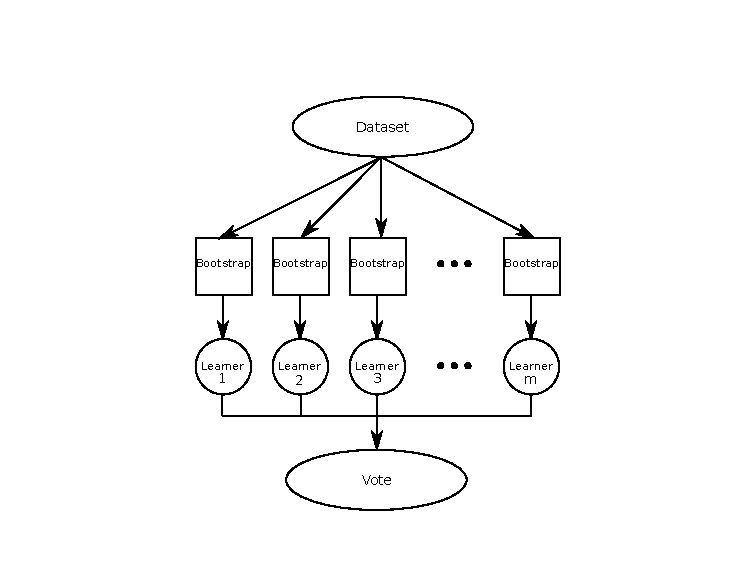
\includegraphics[scale=0.8]{./plots/bagging1.pdf}
        \end{figure}
\end{itemize}
\end{frame}

\begin{frame}{Bootstrap aggregating (bagging)}{Example}
    \begin{figure}
        \only<1>{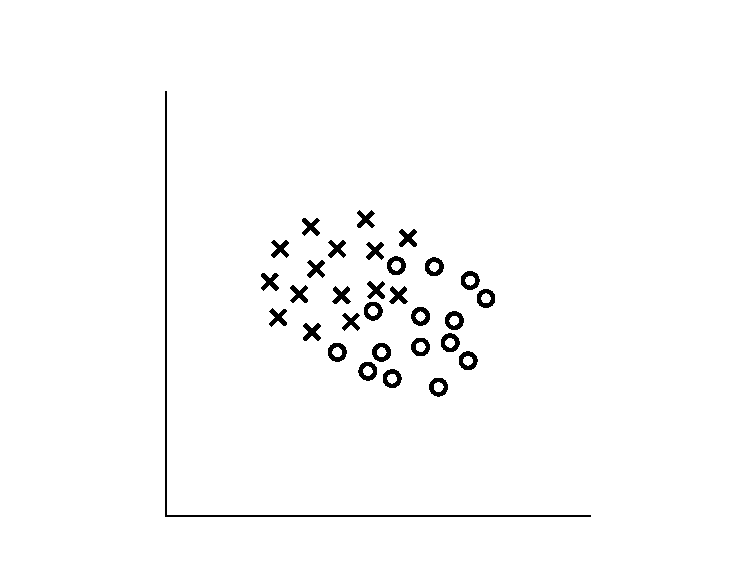
\includegraphics[scale=0.8]{./plots/bagging2.pdf}}
        \only<2>{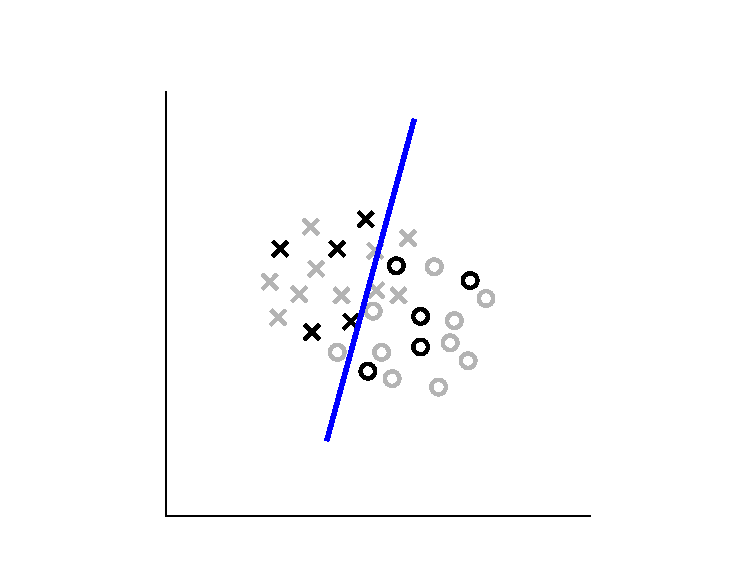
\includegraphics[scale=0.8]{./plots/bagging3.pdf}}
        \only<3>{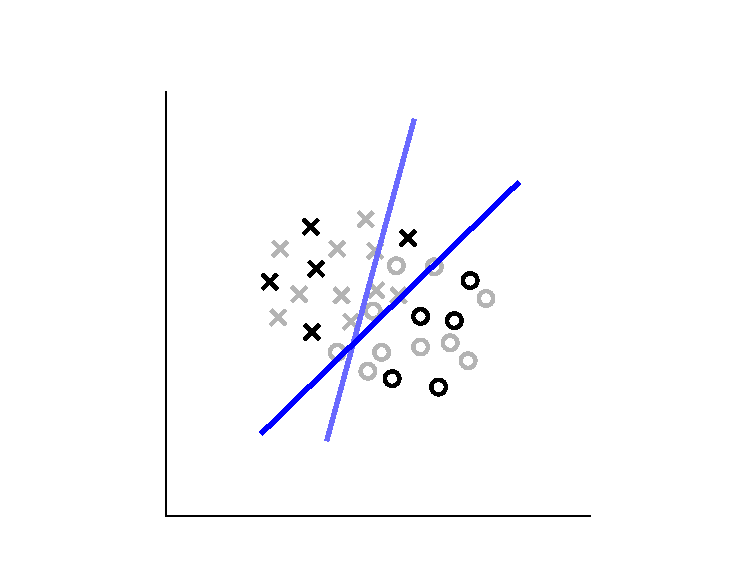
\includegraphics[scale=0.8]{./plots/bagging4.pdf}}
        \only<4>{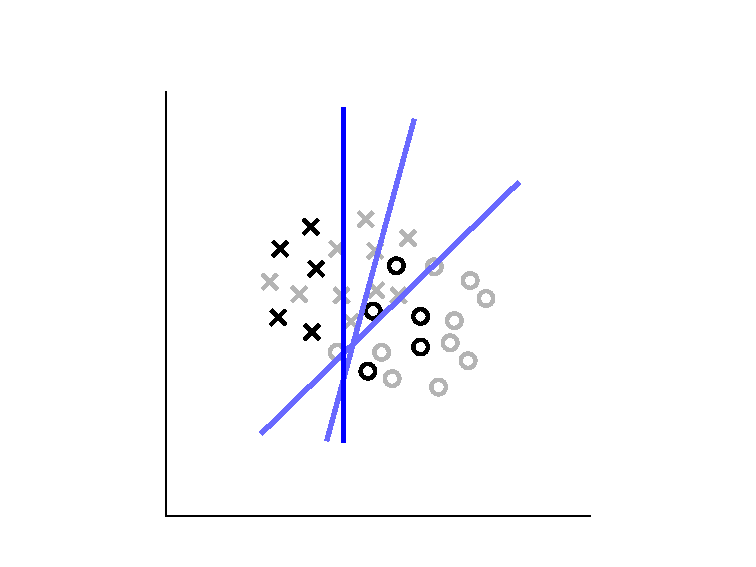
\includegraphics[scale=0.8]{./plots/bagging5.pdf}}
        \only<5>{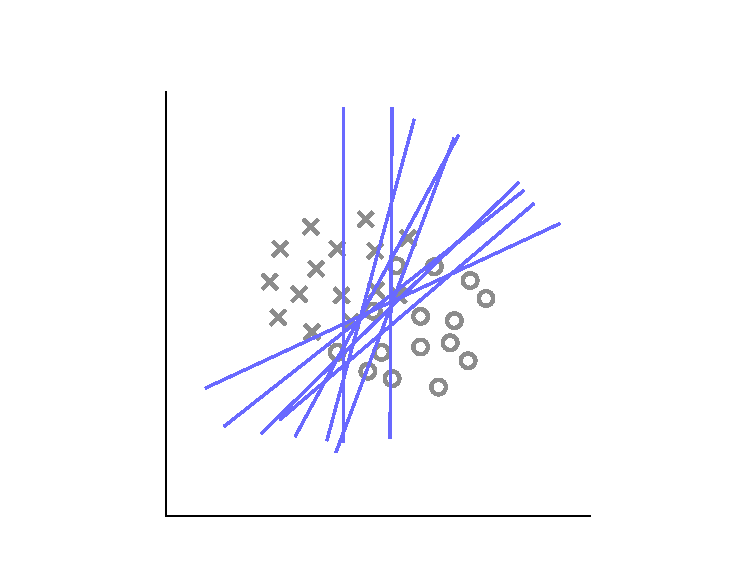
\includegraphics[scale=0.8]{./plots/bagging6.pdf}}
        \only<6>{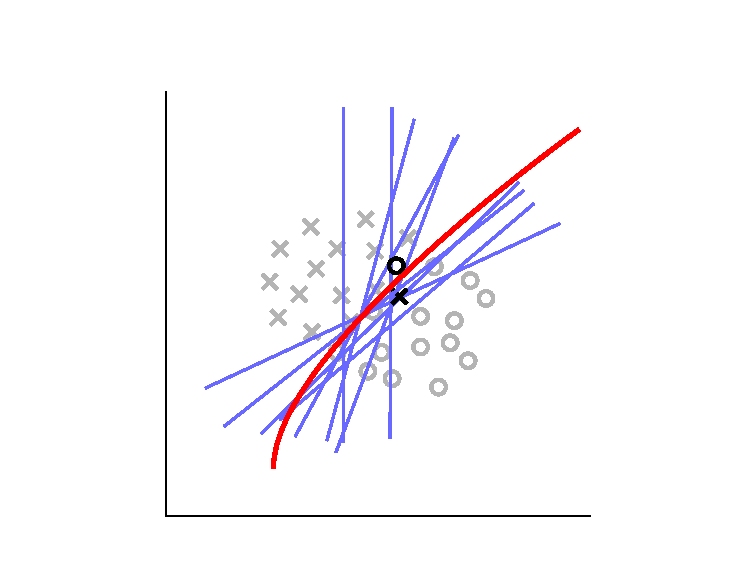
\includegraphics[scale=0.8]{./plots/bagging7.pdf}}
    \end{figure}
\end{frame}

\begin{frame}{Bootstrap aggregating (bagging)}{Why bagging works?}
\begin{itemize}
    \item Suppose there are $25$ base learners
    \item Each has an error rate $\eta=0.35$ 
    \item Assume independence among classifiers
    \item Probability that the ensemble makes a mistake 
    \begin{align*}
        \sum_{i=13}^{25}\left(\begin{array}{c} 25\\i\end{array}\right)\eta^i(1-\eta)^{25-i}=0.06
    \end{align*}
\end{itemize}
\end{frame}


\begin{frame}[allowframebreaks]{Bootstrap aggregating (bagging)}{Bias-Variance Decomposition}
\begin{itemize}
    \item Error of learning algorithm on example $x$ comes from three source
    \begin{itemize}
        \item Noise, measure error / uncertainty for true label of $x$
        \item Bias, how close/good, is the algorithm to optimal prediction
        \item Variance, how much does prediction change if when training data change
    \end{itemize}
    \item Error can be decomposed as:
        \begin{align*}
            error(x)=noise(x)+bias(x)+variance(x)
        \end{align*}
    \item Bias-variance trade-off
    \begin{itemize}
        \item high bias $\mapsto$ low variance
        \item low bias $\mapsto$ high variance
    \end{itemize}
    \item Averaging can decrease variance while have the same bias
    \begin{align*}
    Var(\hat{x}) = \frac{Var(x)}{N}
    \end{align*}
    \item Bagging can be viewed as averaging.
    \item Bagging typically helps
    \begin{itemize}
        \item Over-fitted base model: high variance \& low bias
        \item Unstable model: highly dependent on training data (decision tree, KNN, etc)
    \end{itemize}
\end{itemize}
\end{frame}

%\TODO random forest
\subsection{Boosting}

\begin{frame}{Boosting}
\begin{itemize}
    \item Boosting:
    \begin{itemize}
        \item Base learner is just better than random prediction(coin toss)
        \item Incrementally build an ensemble.
        \item Each new model instant emphasizes the training instances that previous model misclassified.
    \end{itemize}
    \item Adaptive Boosting (Adaboost) \href{run:adaboostmh.pdf}{($\blacksquare$ See additional material)} \cite{Freund92,SchSin98}
    \item Boosting can:
    \begin{itemize}
        \item Reduce variance, like bagging
        \item Eliminate the effect the high bias of the weak learner \cite{FreSch96}
    \end{itemize}
\end{itemize}
\end{frame}


\begin{comment}
\begin{frame}{}
\begin{itemize}
    \item 
\end{itemize}
\end{frame}
\end{comment}


%\subsection{Ensemble of Graph Labeling Classifiers}


\section{Multi-Label/Task Classification}
\begin{frame}{Support Vector Machine Revisit}
\begin{itemize}
    \item Learning Task 
    \begin{itemize}
        \item Single task, binary classification
        \item $m$ examples $\{(x_1,y_{1}),\cdots,(x_m,y_{m})\},x_i\in\mathcal{R}^d,y_i\in\{+,-\}$
    \end{itemize}
    \item Linear separator of the form $f(\xb) = \wb^T \xb + b$
    \item Principal:{\em Empirical risk minimization}
    \begin{itemize}
        \item minimize training error
    \end{itemize}
    \item Hyperplanes with same empirical risk
    \begin{figure}
        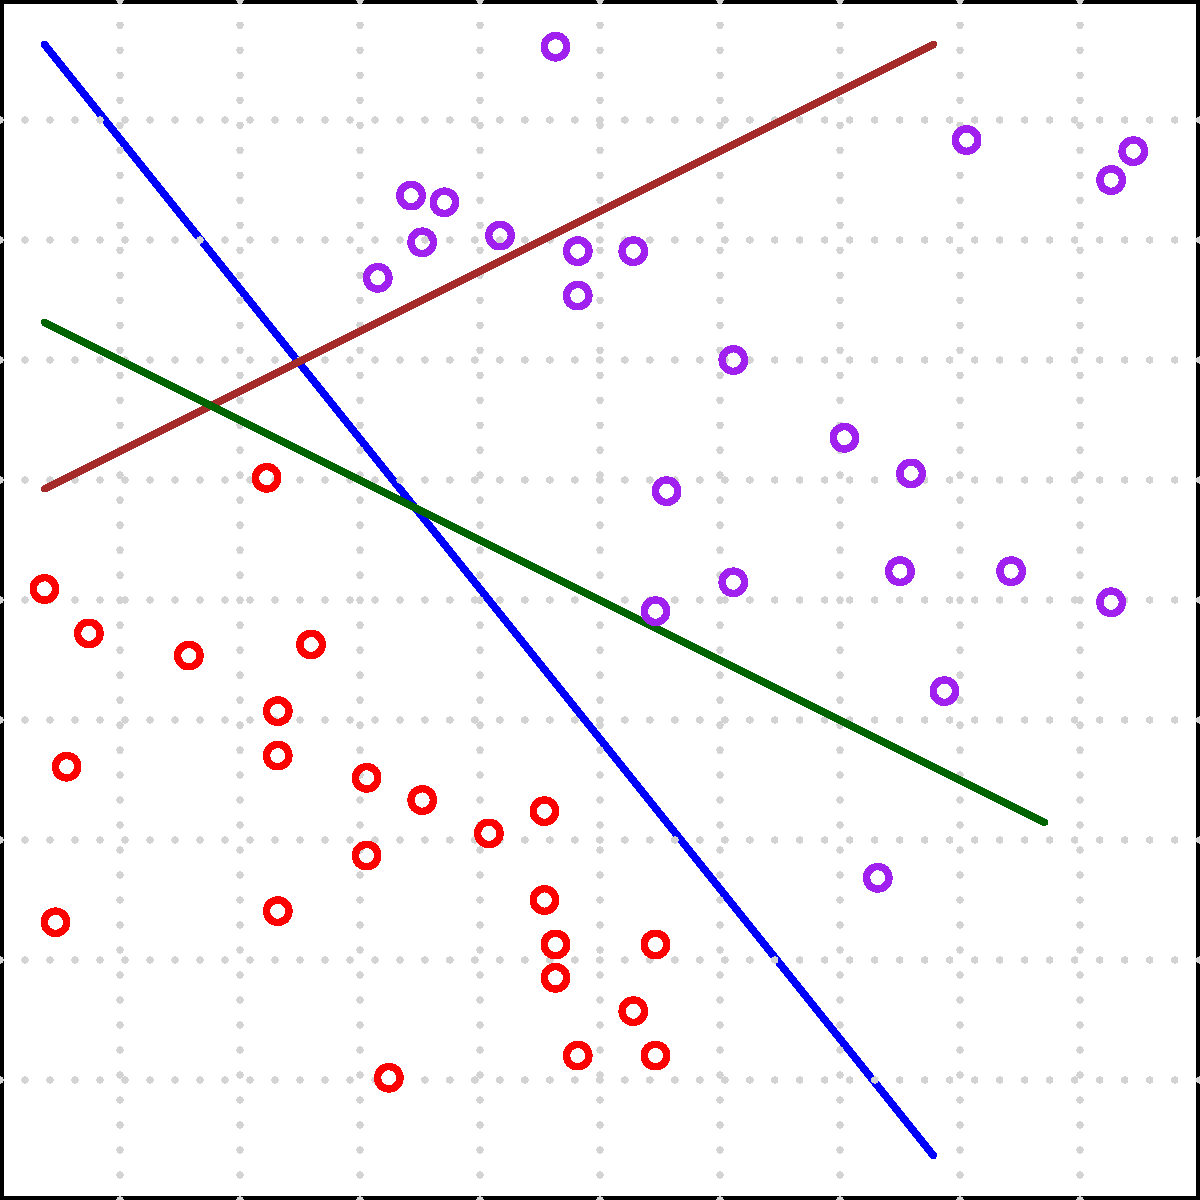
\includegraphics[scale=0.15]{./plots/empirical_risk.pdf}\,
        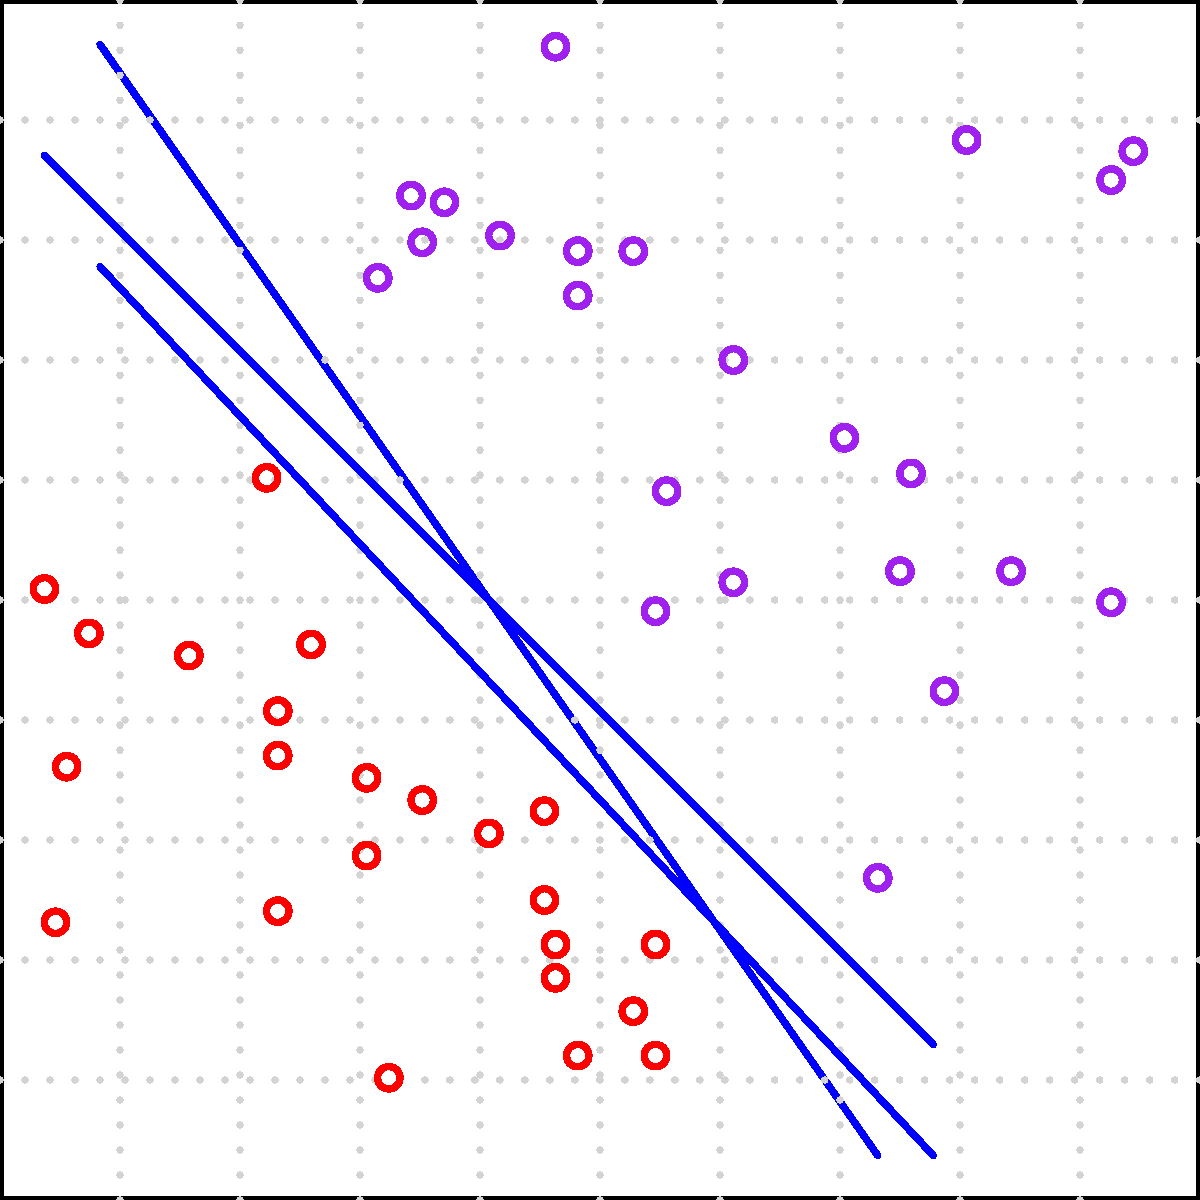
\includegraphics[scale=0.15]{./plots/linear_perceptron.pdf}
    \end{figure}
\end{itemize}
\end{frame}

\begin{frame}{Support Vector Machine Revisit}{Max-Margin Hyperplane}
\begin{itemize}
    \item Maximum margin hyperplane (hard-Margin).
    \begin{itemize}
        \item Robustness: small perturbation in training data does not change the classification
        \item Performance: a large margin leads to low error on unseen data
    \end{itemize}
    \item Hard-Margin SVM takes the form:
    \begin{columns}
        \begin{column}{.5\linewidth}
            \begin{align*}
            (\wb,b) & = \underset{\wb,b}{\operatorname{\argmin}} \, \frac{1}{2} ||\wb||^2,\\
            \text{ s.t. } & y_i\,(\wb^T\xb_i + b) \ge 1,\\
            & 1 \leq i \leq n. \nonumber
            \end{align*}
        \end{column}
        \begin{column}{.5\linewidth}
            \begin{figure}
                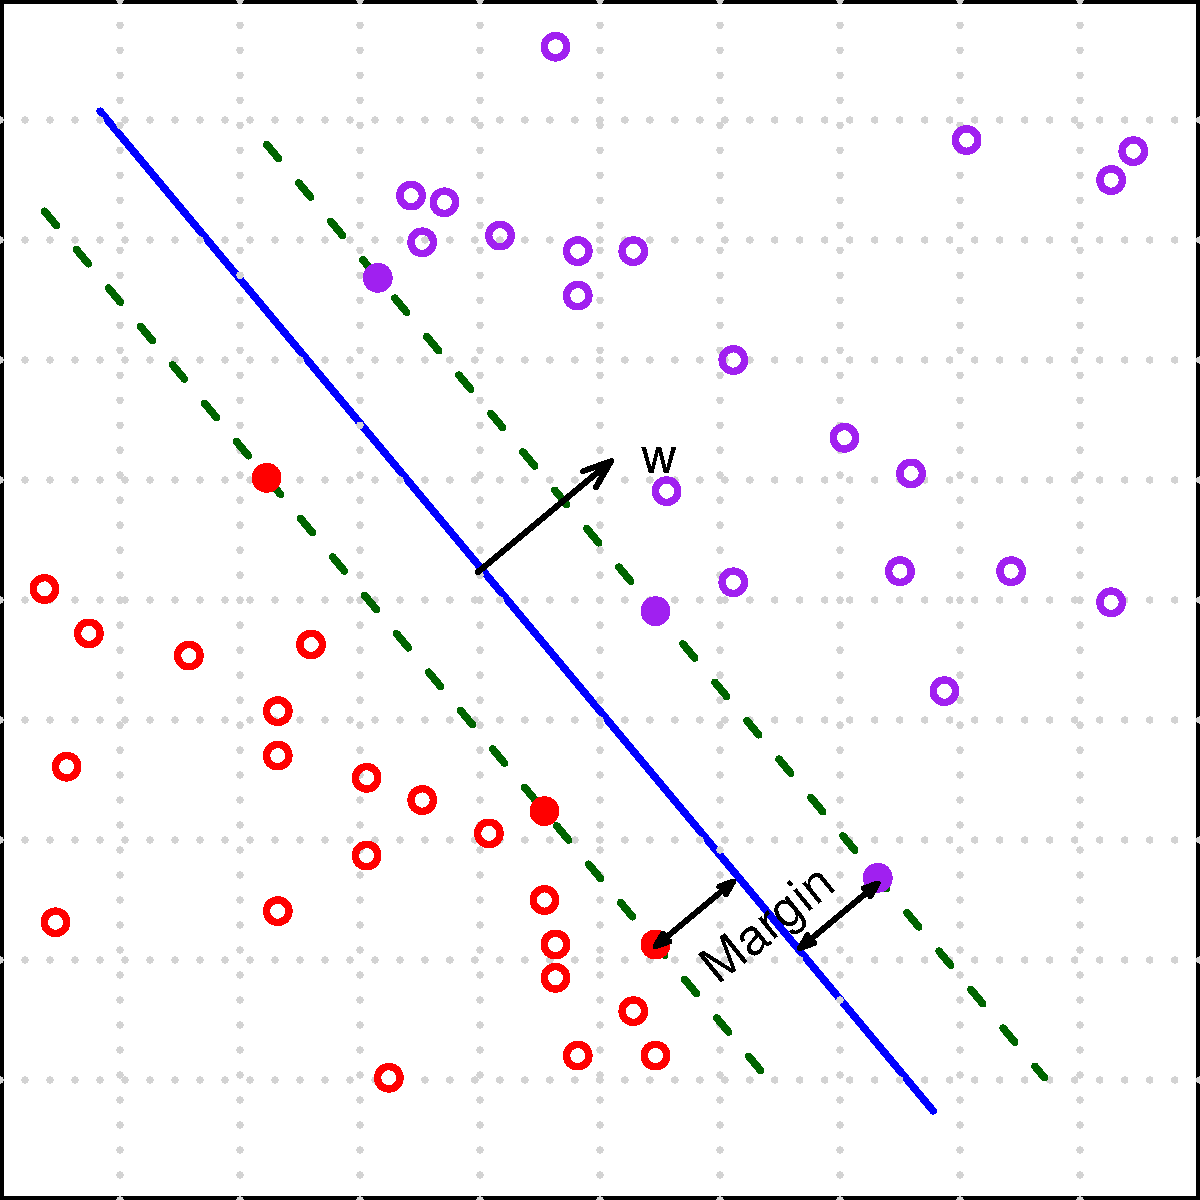
\includegraphics[scale=0.15]{./plots/margin_maximization.pdf}
            \end{figure}
        \end{column}
    \end{columns}
\end{itemize}
\end{frame}

\begin{frame}{Support Vector Machine Revisit}{Soft-Margin SVM \cite{CorVap95}}
\begin{itemize}
    \item In practice, training data cannot be perfectly classified by a hyperplane 
    \item Soft-Margin hyperplane allows training points to have smaller margin, subject to a penalty $\xi$
    \item Soft-Margin SVM takes the form
    \begin{columns}
        \begin{column}{.5\linewidth}
            \begin{align*}
            (\wb,b)  &= \underset{\wb,b}{\operatorname{\argmin}}\left( \frac{1}{2} ||\wb||^2 + C \sum_{i=1}^m \xi_i \right) \text{,}  \\
            \text{ s.t. } & y_i\,(\wb^T \xb_i + b) \ge 1 - \xi_i \text{,}  \\
            & \xi_i \ge 0  \text{, } 1 \leq i \leq n \text{.} 
            \end{align*}
        \end{column}
        \begin{column}{.5\linewidth}
            \begin{figure}
                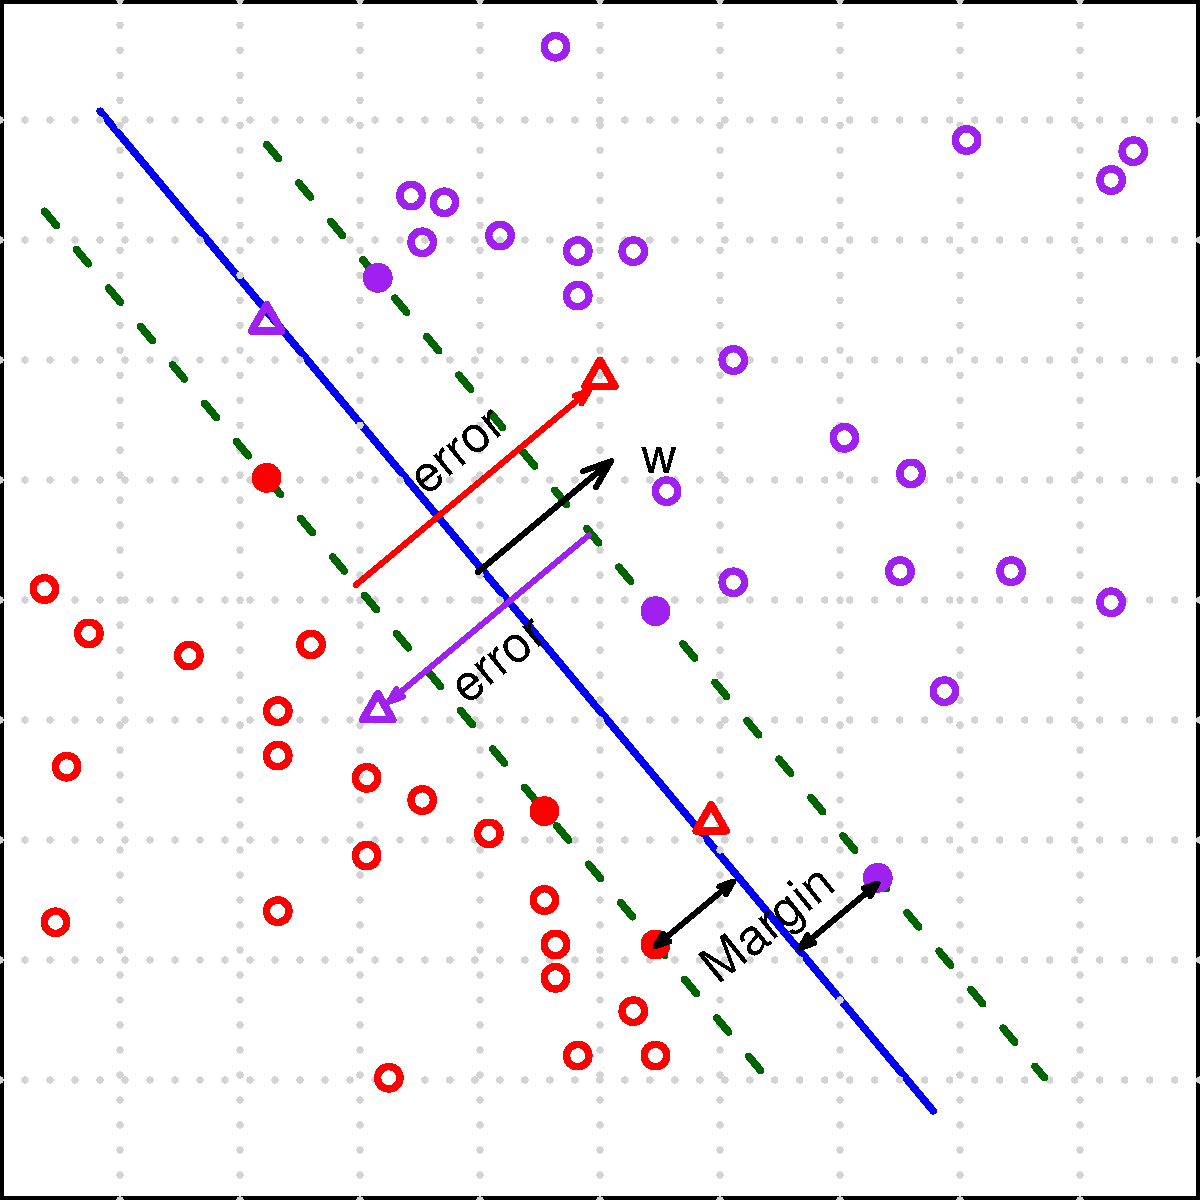
\includegraphics[scale=0.15]{./plots/soft_margin.pdf}
            \end{figure}
        \end{column}
    \end{columns}
\end{itemize}
\end{frame}

\begin{frame}[allowframebreaks]{Support Vector Machine Revisit}{Non-linear SVM}
\begin{itemize}
    \item Training data is not linear separable.
    \begin{figure}
        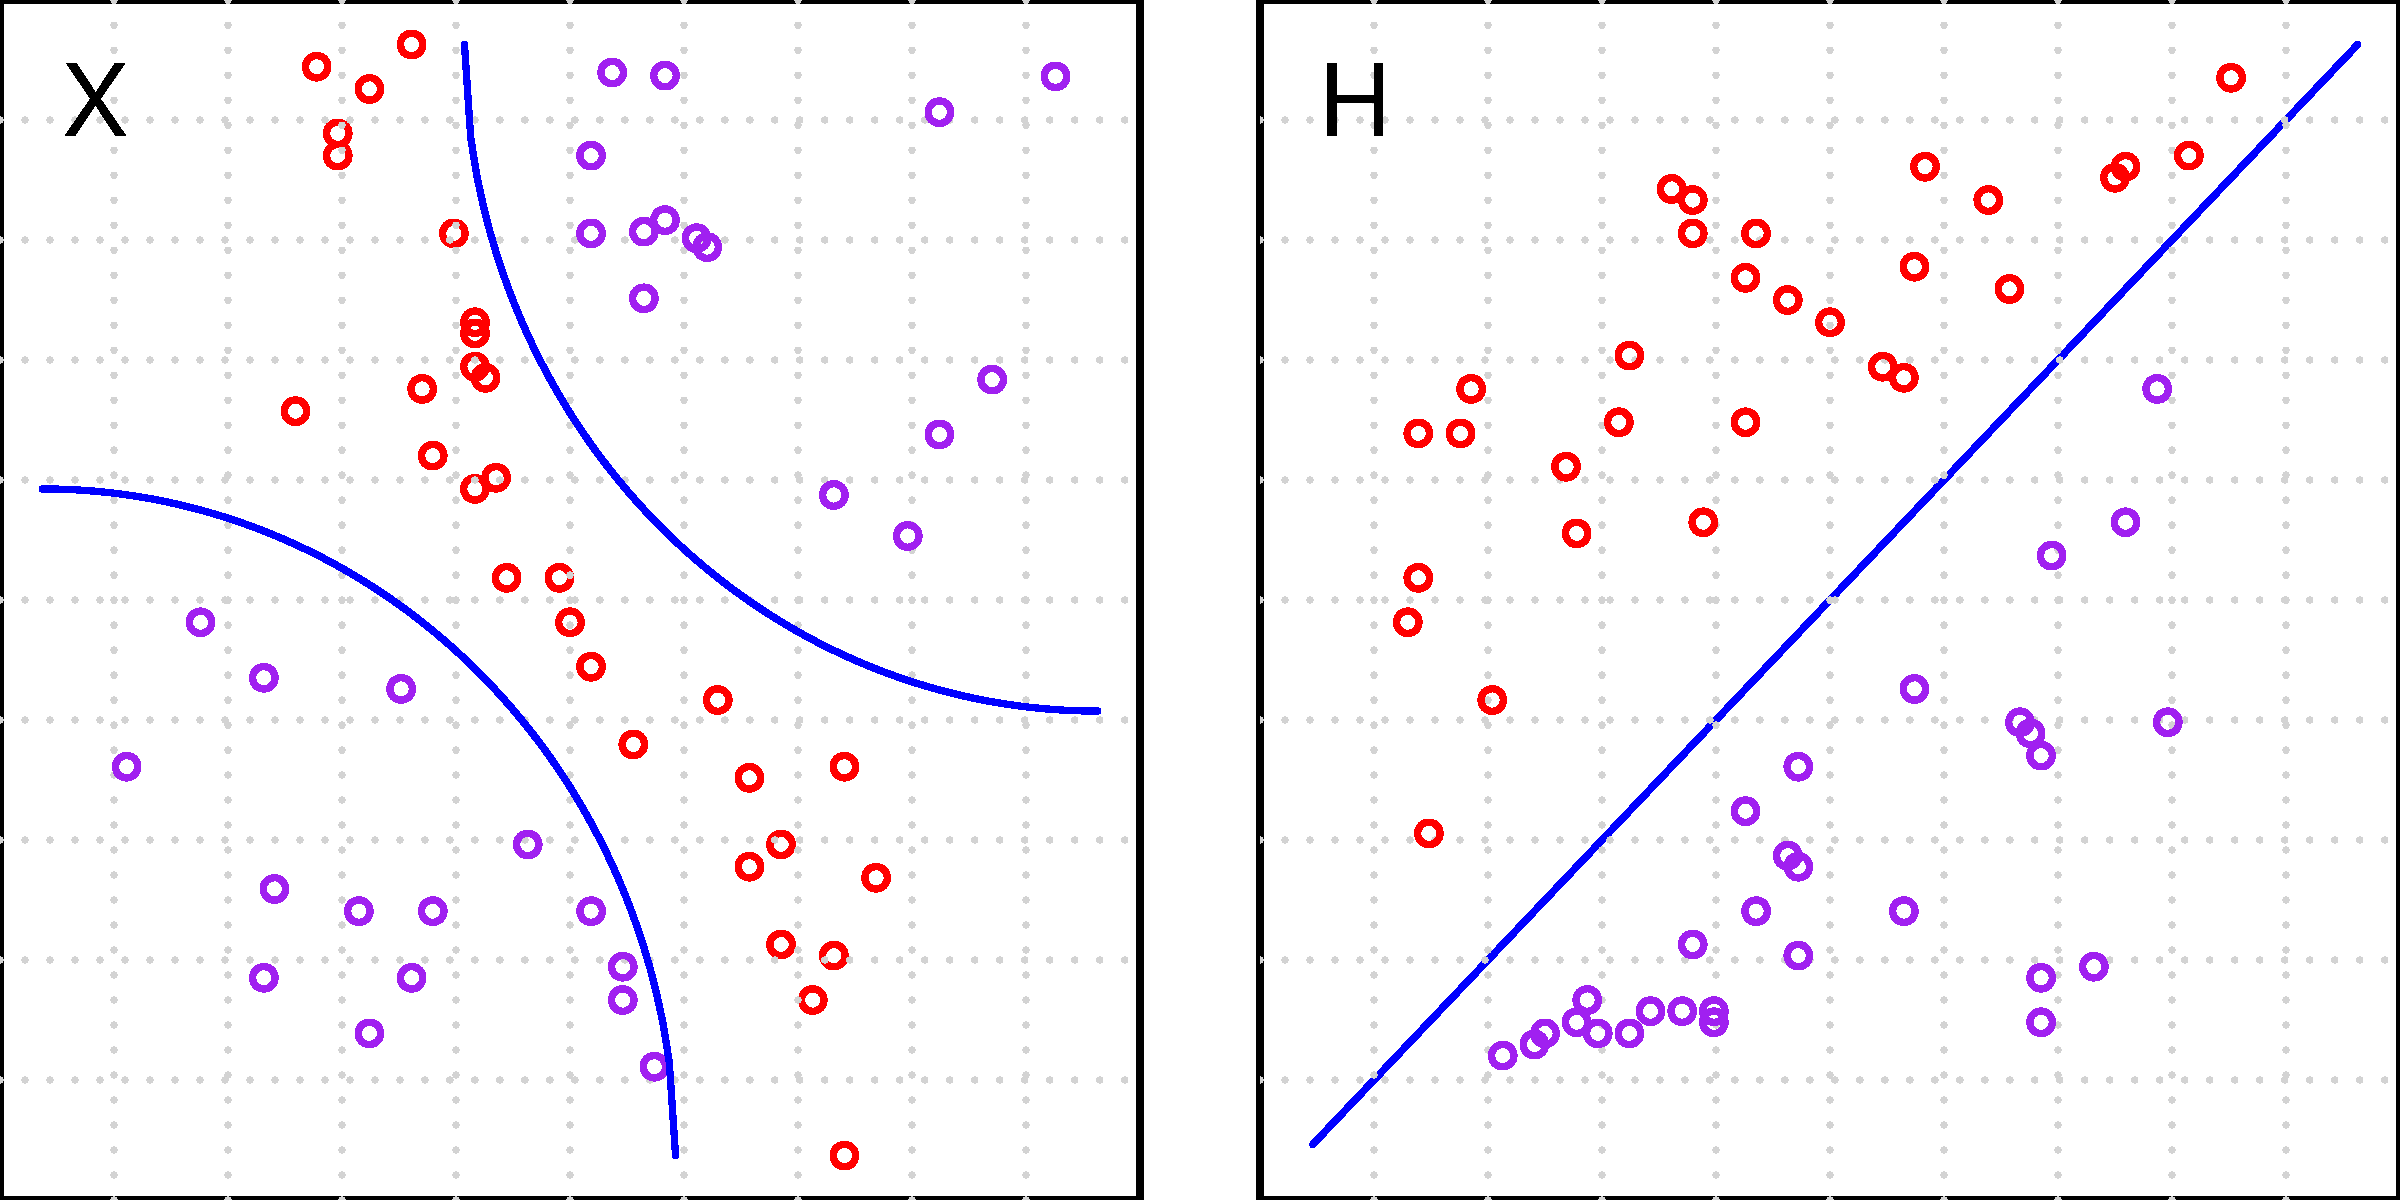
\includegraphics[scale=0.15]{./plots/kernel_svm.pdf}
    \end{figure}
    \item Map data to high dimensional space $\mathcal{H}$, $\xb_i = (x_1,x_2,\cdots,x_n) \xrightarrow{\varphi} \varphi(\xb_i) = (\varphi_1,\varphi_2,\cdots,\varphi_k) \text{.}$
    \item Dual is given by
\begin{align*}
\tilde{\Lcal}(\alpha) = &\sum_{i=1}^{n}{\alpha_i} - \sum_{i = 1}^{n}\sum_{j = 1}^{n}{\alpha_i \alpha_j y_i y_j (\varphi(\xb_i) \cdot \varphi(\xb_j))}\\
= &\sum_{i=1}^{n}{\alpha_i} - \sum_{i = 1}^{n}\sum_{j = 1}^{n}{\alpha_i \alpha_j y_i y_j K(\xb_i,\xb_j)}
\end{align*}
    \item kernel trick: mapping observation to inner product space without computing the mappping explicitly.
    \item Example
\begin{itemize}
\item Assume we have variables $X$ and $Y$ in $n$ dimensional feature space $X,Y \in \mathbb{R}^n$

\begin{align}
\phi(X) &= (x_1, \ldots,x_n) \\
\phi(Y) &= (y_1, \ldots, y_n) 
\end{align}

Linear kernel corresponds to a dot product denoted by

\begin{align}
K_{linear}(X,Y) &=  \phi(X) \cdot \phi(Y) \\
 &= \sum_i^n x_i y_i
\end{align}

A more interesting kernel can be constructed by constructing a kernel from two different feature sets $\phi_A(X) \in \mathbb{R}^a$ and $\phi_B(X) \in \mathbb{R}^b$. We can combine the two feature sets into $a+b$ dimensional vector $\phi_{A,B}(X) = [\phi_A(X), \phi_B(X)]$ and computing the kernel $K_{A,B}(X,Y)$ directly as $\phi_{A,B}(X)\cdot \phi_{A,B}(Y)$. However, by definition $K_A(X,Y) + K_B(X,Y) = K_{A,B}(X,Y)$. Thus, we can either concatenate features before hand and then compute a single kernel, or compute the individual kernels and sum them.

By taking an element-wise product $K_A \cdot K_B$ between kernels $K_A$ and $K_B$ we get features of type $\phi_A(X)_i \phi_B(X)_j$ for all $i \in [1,\ldots, a]$ and $j \in [1, \ldots, b]$.

For quadratic kernels, we have

\begin{align}
K_{quadratic}(X,Y) &= (K_{linear}(X,Y) + C)^2 \\
 &= \left( \sum_i^n x_i y_i + C \right)^2 \\
 &= \sum_{i=1}^n \sum_{j=1}^n x_i x_j y_i y_j + 2 \sum_{i=1}^n x_i y_i + C^2 \\
 &= \sum_{i=1}^n \sum_{j=1}^n x_i x_j y_i y_j + \sum_{i=1}^n \sqrt{2} x_i \sqrt{2} y_i + C^2 \\
 &= \phi'(X) \cdot \phi'(Y),
\end{align}

where the expanded feature spaces $\phi'(X)$ and $\phi'(Y)$ are

\begin{align}
\phi'(X) &= (x_1 x_1, \ldots, x_1 x_n, x_2 x_1, \ldots, x_n x_n; \sqrt{2} x_1, \ldots, \sqrt{2} x_n, C) \\
\phi'(Y) &= (y_1 y_1, \ldots, y_1 y_n, y_2 y_1, \ldots, y_n y_n; \sqrt{2} y_1, \ldots, \sqrt{2} y_n, C) 
\end{align}
\end{itemize}

\end{itemize}
\end{frame}

\begin{frame}[allowframebreaks]{Structured Multi-Task Classification}
\begin{itemize}
    \item $m$ training data $\{(x_i,\yb_i)\}_{i=1}^m$
    \item $d$ dimension feature representation for each example $x\in\mathcal{R}^d$
    \item $T$ targets/labels, $\yb\in\{+,-\}^T$
    \item General form:
    \begin{align*}
    X &= \left[ 
    \begin{array}{ccccc} 
    x_{11}&x_{12}&\ldots &x_{1d}\\ 
    \vdots&\vdots&\ddots&\vdots\\ 
    \mathbf{x_{i1}}&\mathbf{x_{i2}}&\ldots &\mathbf{x_{id}}\\ 
    \vdots&\vdots&\ddots&\vdots\\ 
    x_{m1}&x_{m2}&\ldots &x_{md}\\ 
    \end{array} 
    \right],
    &Y =& \left[ 
    \begin{array}{cccc} 
    y_{11}&y_{12}&\ldots &y_{1T}\\ 
    \vdots&\vdots&\ddots&\vdots\\ 
    \mathbf{y_{i1}}&\mathbf{y_{i2}}&\ldots &\mathbf{y_{iT}}\\ 
    \vdots&\vdots&\ddots&\vdots\\ 
    y_{m1}&y_{m2}&\ldots &y_{mT}\\ 
    \end{array} 
    \right]\\
    {x_j} &= \left( 
    \begin{array}{ccccc} 
    {x}_{j1}&{x}_{j2}&\ldots &{x}_{jm}\\
    \end{array} 
    \right),
    &{y_j} =& \left(
    \begin{array}{cccc} 
    ?&?&\cdots&?\\
    \end{array} 
    \right)
    \end{align*}
    \framebreak
    \item Output graph: a structure $\mathcal{G}=(E,V)$ on multiple targets
    \begin{itemize}
        \item A node $v\in V$ corresponds to target/label
        \item An edge $e\in E$ represents dependency between pair of targets  
    \end{itemize}
    \item A prediction of multiple targets/labels can be seen as a labeling of the output graph.
    \begin{figure}
        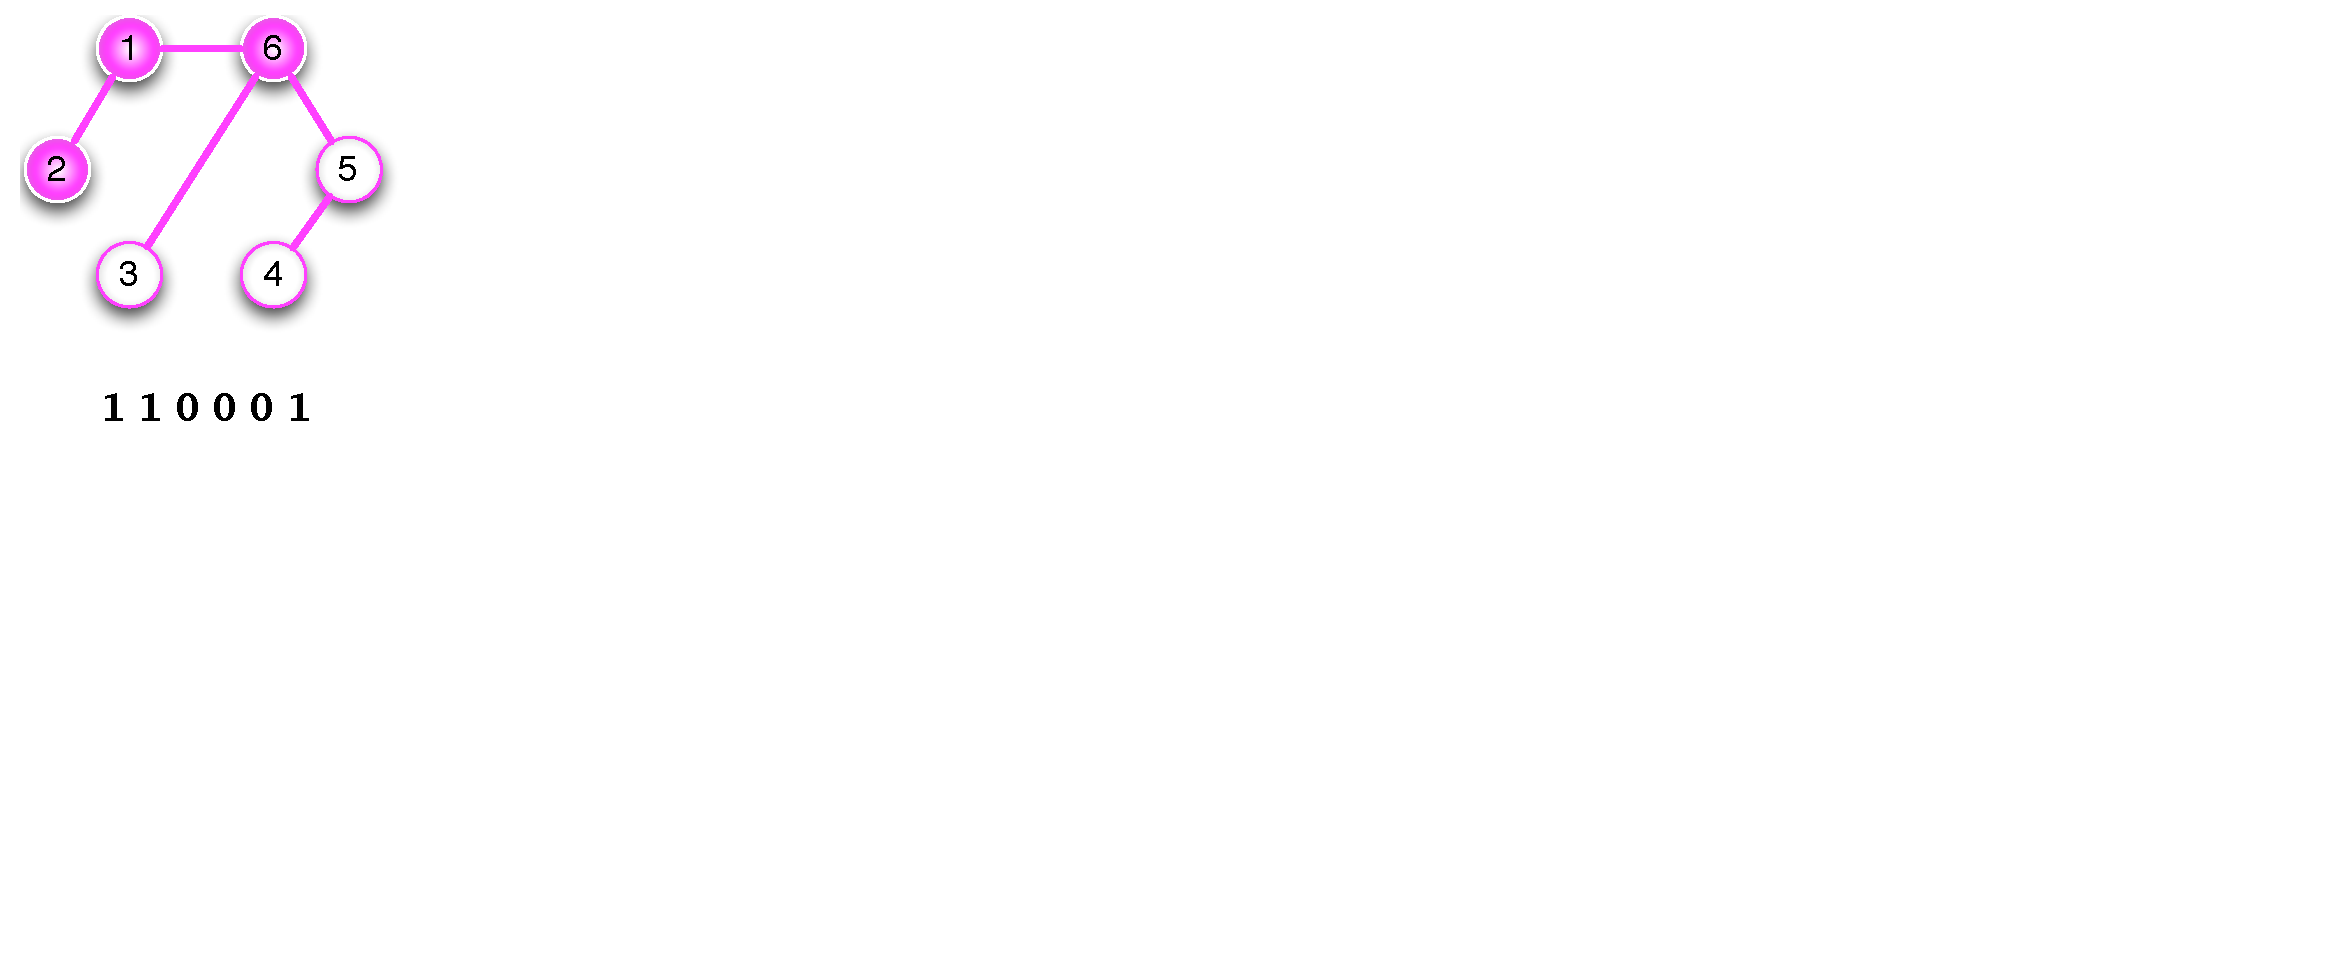
\includegraphics[scale=.3]{./plots/graphlabeling.pdf}
    \end{figure}
        $\yb=(y_1,y_2,y_3,y_4,y_5,y_6)$
\end{itemize}
\end{frame}


\begin{frame}[allowframebreaks]{Application Areas }
\begin{itemize}
    \item Hierarchical document classification \cite{veeramachaneni2005hierarchical,eps262947} 
    \begin{columns}
        \begin{column}{.5\linewidth}
            Given news articles $x$ and the classification hierarchy $\mathcal{G}$, predict the multiple categories of the new article. 
        \end{column}
        \begin{column}{.5\linewidth}
            \begin{figure}
                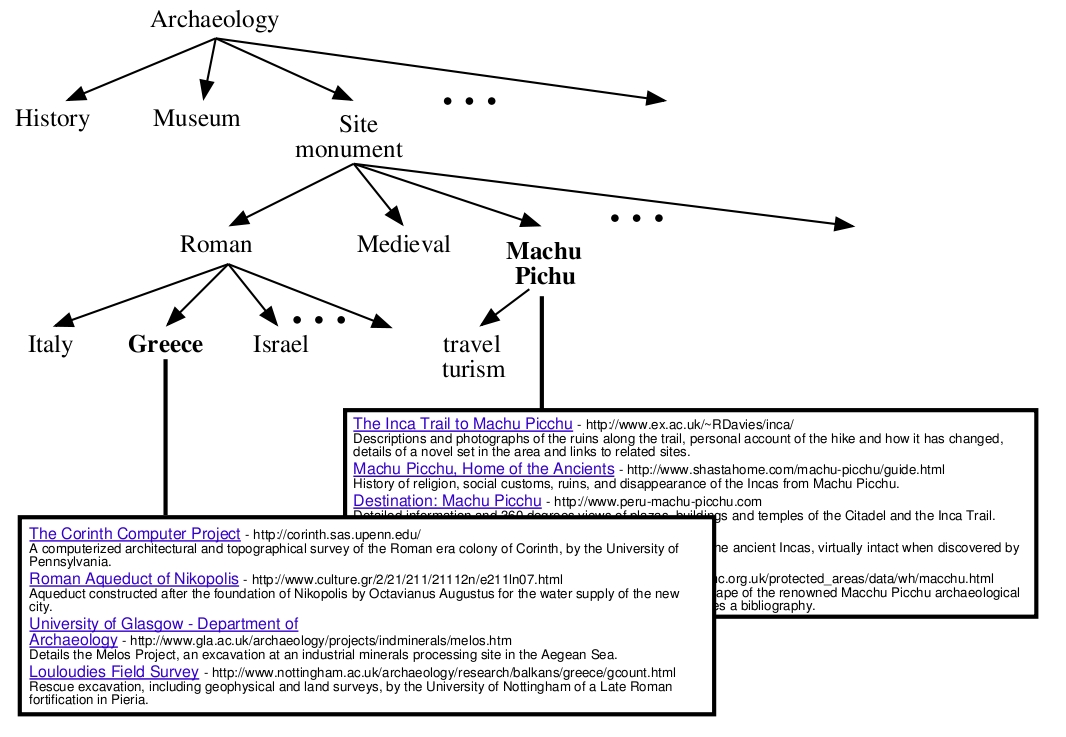
\includegraphics[scale=0.2]{./plots/document.jpg}
            \end{figure}
        \end{column}
    \end{columns}
    \framebreak
    \item Medical diagnosis \cite{Huang13042010}\\ 
        Given microarray profile of tissue sample $x$ and the disease hierarchy $\mathcal{G}$, predict multiple labels in the hierarchy.
        \begin{figure}
            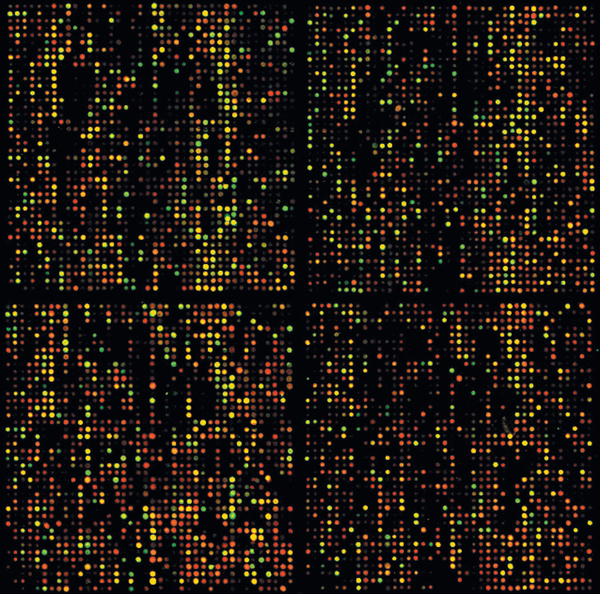
\includegraphics[scale=0.08]{./plots/microarray.jpg}\,
            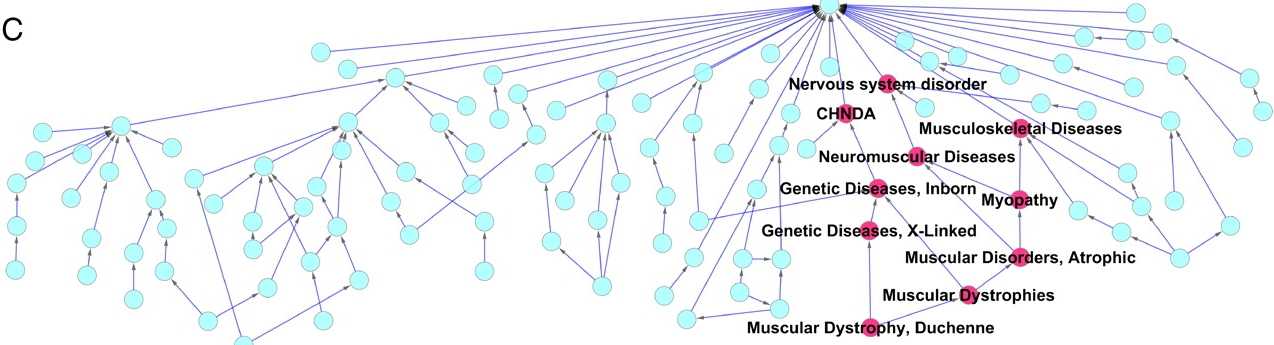
\includegraphics[scale=0.18]{./plots/umls.jpg}
        \end{figure}
    \framebreak
     \begin{columns}
        \begin{column}{.6\linewidth}
    \item Drug bioactivity prediction \cite{su2010}\\ 
        Given molecular structure $x$ and relation of cancer cell lines, predict the anti-cancer potentials of the molecules.
        \end{column}
        \begin{column}{.3\linewidth}
        \begin{figure}
        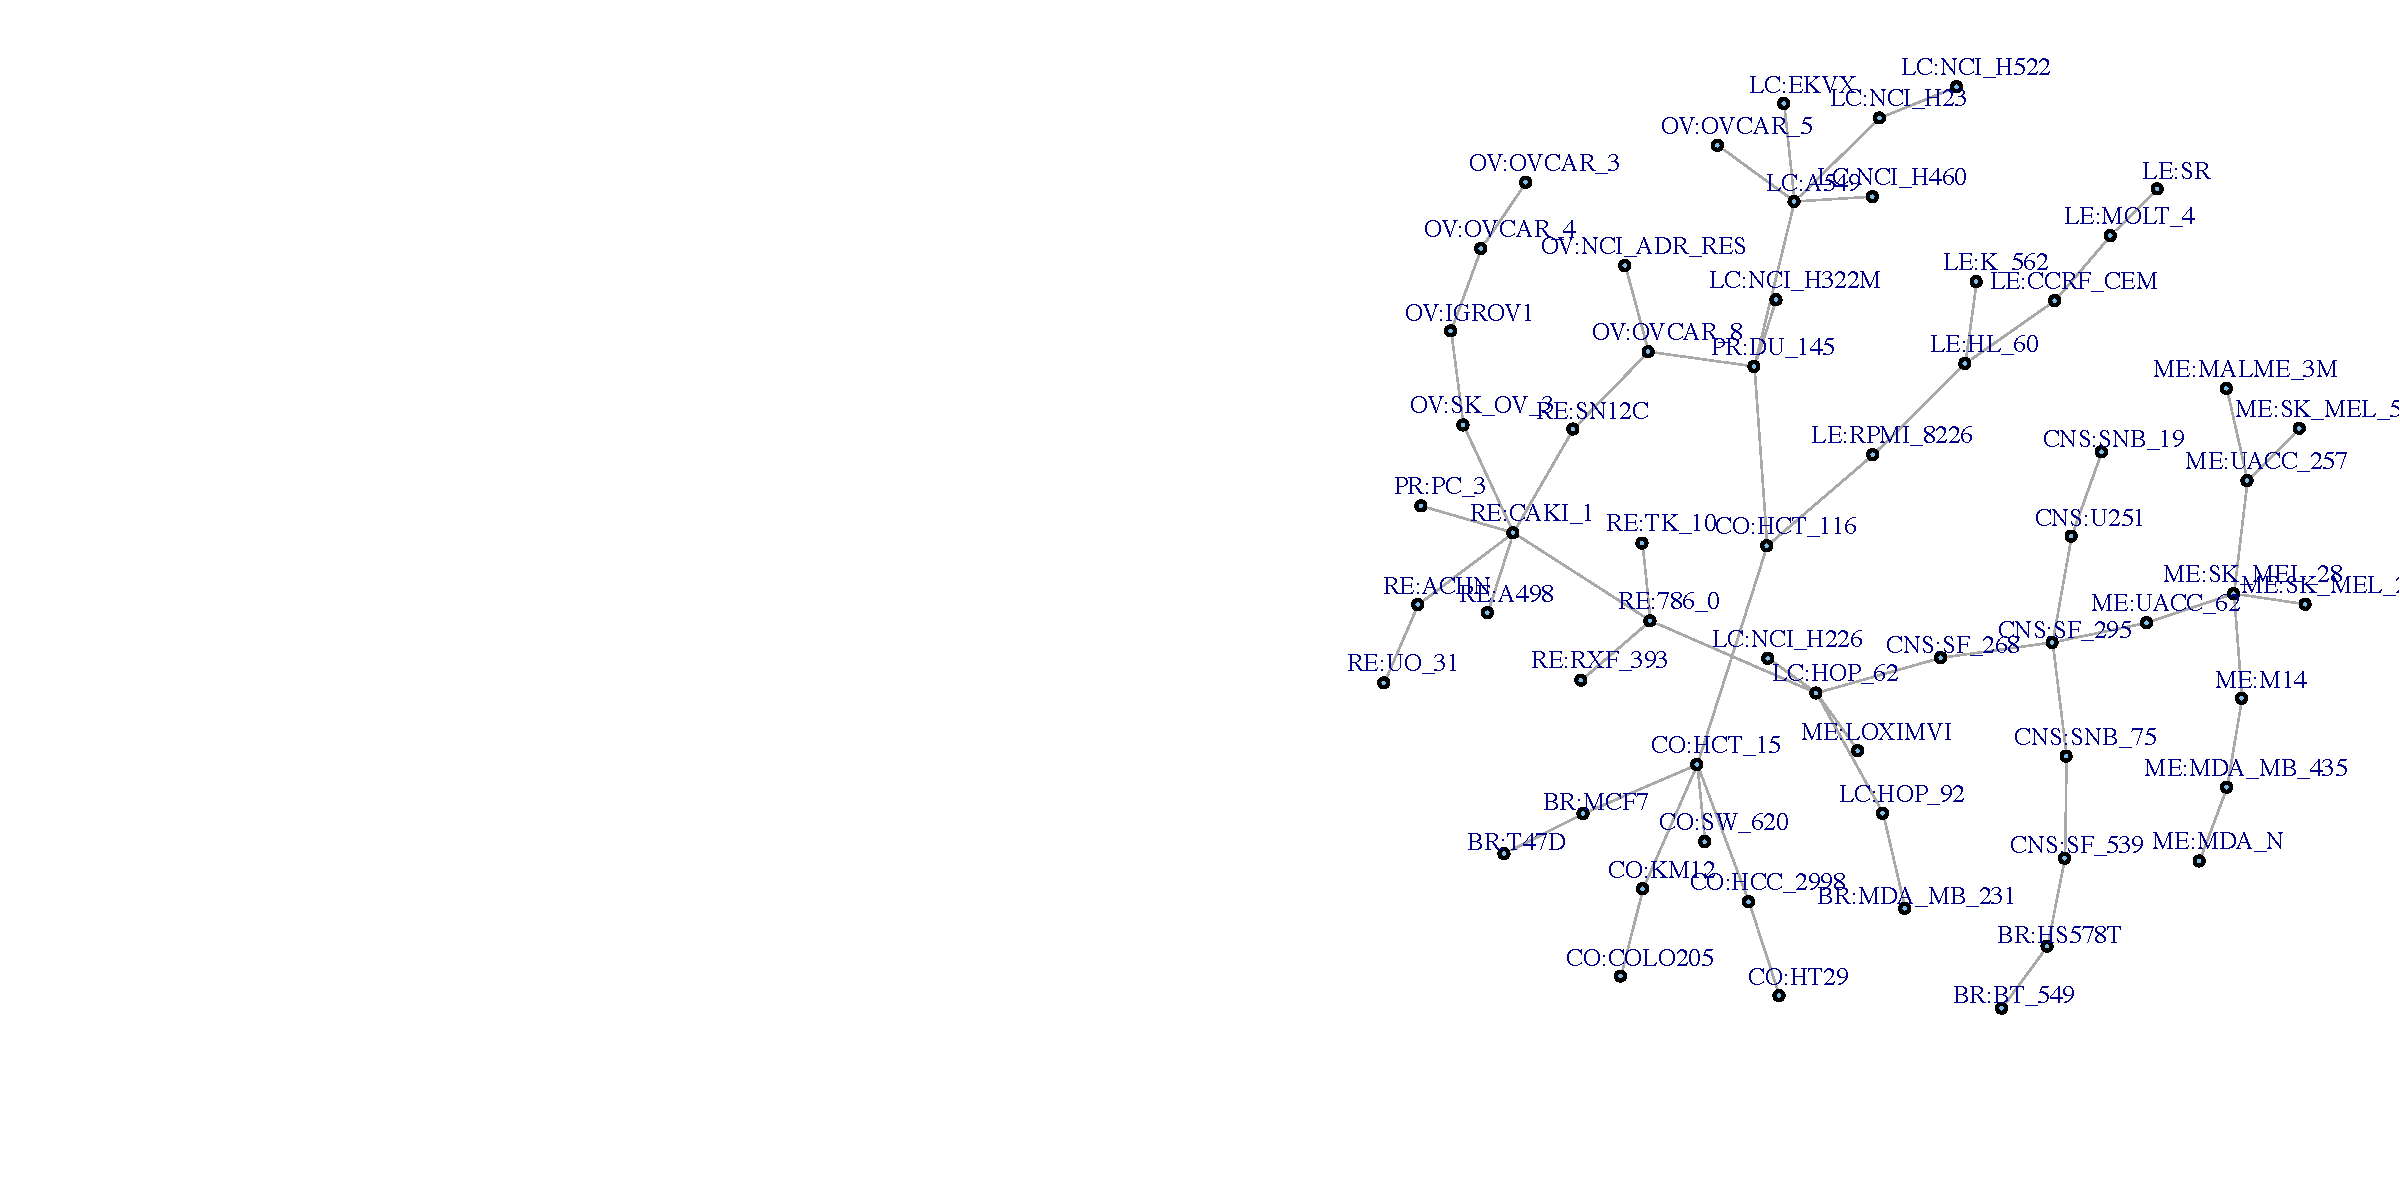
\includegraphics[scale=0.2]{./plots/cancernet.pdf}
        \end{figure} 
        \end{column}
    \end{columns}
            \begin{align*}
            x \xrightarrow{\blue predict} \mathbf{y} = \{y_1,y_2,\cdots,y_{60}\}, y_i \in \{0,1\}.
            \end{align*}
            \begin{center}
            {\only<1>
            {\begin{table}
            \scriptsize
            \begin{tabular}{p{1cm}p{0.08cm}p{0.08cm}p{0.08cm}p{0.08cm}p{0.08cm}p{0.08cm}p{0.08cm}p{0.08cm}p{0.08cm}p{0.08cm}p{0.08cm}p{0.08cm}p{0.08cm}p{0.08cm}p{0.08cm}p{0.08cm}}
            \multirow{4}{*}{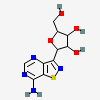
\includegraphics[scale = 0.3]{./plots/mol1.png}} & 
            \cellcolor{purple}1&\cellcolor{purple}1&\cellcolor{purple}1&\cellcolor{purple}1&\cellcolor{purple}1&\cellcolor{purple}1&\cellcolor{purple}1&\cellcolor{purple}1&\cellcolor{purple}1&\cellcolor{purple}1&\cellcolor{purple}1&\cellcolor{purple}1&\cellcolor{purple}1&\cellcolor{purple}1&\cellcolor{purple}1 \\ 
            &\cellcolor{purple}1&\cellcolor{purple}1&\cellcolor{purple}1&\cellcolor{purple}1&\cellcolor{purple}1&\cellcolor{blue}0&\cellcolor{purple}1&\cellcolor{purple}1&\cellcolor{purple}1&\cellcolor{purple}1&\cellcolor{blue}0&\cellcolor{purple}1&\cellcolor{purple}1&\cellcolor{purple}1&\cellcolor{purple}1 \\ 
            &\cellcolor{purple}1&\cellcolor{purple}1&\cellcolor{purple}1&\cellcolor{blue}0&\cellcolor{purple}1&\cellcolor{purple}1&\cellcolor{purple}1&\cellcolor{blue}0&\cellcolor{purple}1&\cellcolor{purple}1&\cellcolor{purple}1&\cellcolor{purple}1&\cellcolor{blue}0&\cellcolor{purple}1&\cellcolor{purple}1 \\ 
            &\cellcolor{purple}1&\cellcolor{purple}1&\cellcolor{purple}1&\cellcolor{purple}1&\cellcolor{purple}1&\cellcolor{purple}1&\cellcolor{purple}1&\cellcolor{purple}1&\cellcolor{blue}0&\cellcolor{purple}1&\cellcolor{purple}1&\cellcolor{purple}1&\cellcolor{purple}1&\cellcolor{purple}1&\cellcolor{purple}1 \\ 
            \end{tabular}
            \end{table}}
            \only<2>
            {\begin{table}
            \scriptsize
            \begin{tabular}{p{1cm}p{0.08cm}p{0.08cm}p{0.08cm}p{0.08cm}p{0.08cm}p{0.08cm}p{0.08cm}p{0.08cm}p{0.08cm}p{0.08cm}p{0.08cm}p{0.08cm}p{0.08cm}p{0.08cm}p{0.08cm}p{0.08cm}}
            \multirow{4}{*}{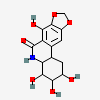
\includegraphics[scale = 0.3]{./plots/mol2.png}} & 
            \cellcolor{purple}1&\cellcolor{blue}0&\cellcolor{blue}0&\cellcolor{blue}0&\cellcolor{blue}0&\cellcolor{blue}0&\cellcolor{blue}0&\cellcolor{purple}1&\cellcolor{blue}0&\cellcolor{blue}0&\cellcolor{blue}0&\cellcolor{blue}0&\cellcolor{blue}0&\cellcolor{blue}0&\cellcolor{blue}0 \\ 
            &\cellcolor{blue}0&\cellcolor{purple}1&\cellcolor{blue}0&\cellcolor{blue}0&\cellcolor{blue}0&\cellcolor{purple}1&\cellcolor{blue}0&\cellcolor{blue}0&\cellcolor{blue}0&\cellcolor{blue}0&\cellcolor{blue}0&\cellcolor{blue}0&\cellcolor{blue}0&\cellcolor{blue}0&\cellcolor{blue}0 \\ 
            &\cellcolor{blue}0&\cellcolor{blue}0&\cellcolor{purple}1&\cellcolor{blue}0&\cellcolor{blue}0&\cellcolor{blue}0&\cellcolor{blue}0&\cellcolor{blue}0&\cellcolor{blue}0&\cellcolor{purple}1&\cellcolor{blue}0&\cellcolor{blue}0&\cellcolor{purple}1&\cellcolor{blue}0&\cellcolor{blue}0 \\ 
            &\cellcolor{blue}0&\cellcolor{blue}0&\cellcolor{blue}0&\cellcolor{blue}0&\cellcolor{blue}0&\cellcolor{blue}0&\cellcolor{blue}0&\cellcolor{purple}1&\cellcolor{blue}0&\cellcolor{blue}0&\cellcolor{blue}0&\cellcolor{blue}0&\cellcolor{blue}0&\cellcolor{blue}0&\cellcolor{purple}1 \\ 
            \end{tabular}
            \end{table}}
            %\only<3>
            %{\begin{table}
            %\scriptsize
            %\begin{tabular}{p{1cm}p{0.08cm}p{0.08cm}p{0.08cm}p{0.08cm}p{0.08cm}p{0.08cm}p{0.08cm}p{0.08cm}p{0.08cm}p{0.08cm}p{0.08cm}p{0.08cm}p{0.08cm}p{0.08cm}p{0.08cm}p{0.08cm}}
            %\multirow{4}{*}{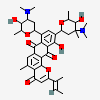
\includegraphics[scale = 0.3]{./plots/mol3.png}} & 
            %\cellcolor{purple}1&\cellcolor{purple}1&\cellcolor{blue}0&\cellcolor{purple}1&\cellcolor{purple}1&\cellcolor{blue}0&\cellcolor{purple}1&\cellcolor{purple}1&\cellcolor{blue}0&\cellcolor{purple}1&\cellcolor{blue}0&\cellcolor{blue}0&\cellcolor{blue}0&\cellcolor{blue}0&\cellcolor{purple}1 \\ 
            %&\cellcolor{purple}1&\cellcolor{blue}0&\cellcolor{blue}0&\cellcolor{purple}1&\cellcolor{purple}1&\cellcolor{blue}0&\cellcolor{blue}0&\cellcolor{purple}1&\cellcolor{blue}0&\cellcolor{blue}0&\cellcolor{purple}1&\cellcolor{blue}0&\cellcolor{purple}1&\cellcolor{purple}1&\cellcolor{blue}0 \\ 
            %&\cellcolor{blue}0&\cellcolor{blue}0&\cellcolor{purple}1&\cellcolor{blue}0&\cellcolor{purple}1&\cellcolor{blue}0&\cellcolor{blue}0&\cellcolor{purple}1&\cellcolor{purple}1&\cellcolor{blue}0&\cellcolor{purple}1&\cellcolor{purple}1&\cellcolor{blue}0&\cellcolor{blue}0&\cellcolor{blue}0 \\ 
            %&\cellcolor{blue}0&\cellcolor{blue}0&\cellcolor{purple}1&\cellcolor{purple}1&\cellcolor{purple}1&\cellcolor{blue}0&\cellcolor{blue}0&\cellcolor{purple}1&\cellcolor{purple}1&\cellcolor{purple}1&\cellcolor{blue}0&\cellcolor{blue}0&\cellcolor{purple}1&\cellcolor{purple}1&\cellcolor{purple}1 \\ 
            %\end{tabular}
            %\end{table}}
            }
            {\footnotesize blocks correspond to cell lines}
        \end{center}
\end{itemize}
\end{frame}

\subsection{via Single-Task Classifier}
\begin{frame}{A Collection of Single-Task Classifiers}
\begin{itemize}
    \item Reduce multiple tasks to a a bag of single takes and solved by a collection of single-task classifiers (e.g. SVM)
   \begin{align*}
    X &= \left[ 
    \begin{array}{ccccc} 
    x_{11}&x_{12}&\ldots &x_{1m}\\ 
    \vdots&\vdots&\ddots&\vdots\\ 
    x_{i1}&x_{i2}&\ldots &x_{im}\\ 
    \vdots&\vdots&\ddots&\vdots\\ 
    x_{n1}&x_{n2}&\ldots &x_{nm}\\ 
    \end{array} 
    \right],
    \only<1>{
    &Y =& \left[ 
    \begin{array}{cccc}
    y_{11}&y_{12}&\ldots &y_{1k}\\ 
    \vdots&\vdots&\ddots&\vdots\\ 
    y_{i1}&y_{i2}&\ldots &y_{ik}\\ 
    \vdots&\vdots&\ddots&\vdots\\ 
    y_{n1}&y_{n2}&\ldots &y_{nk}\\ 
    \end{array} 
    \right]}
    \only<2>{
    &Y =& \left[ 
    \begin{array}{cccc} 
    y_{11}&\ldots&\ldots &\ldots\\ 
    \vdots&\vdots&\ddots&\vdots\\ 
    y_{i1}&\ldots&\ldots &\ldots\\ 
    \vdots&\vdots&\ddots&\vdots\\ 
    y_{n1}&\ldots&\ldots &\ldots\\ 
    \end{array} 
    \right]}
    \only<3>{
    &Y =& \left[ 
    \begin{array}{cccc} 
    \ldots&y_{12}&\ldots &\ldots\\ 
    \vdots&\vdots&\ddots&\vdots\\ 
    \ldots&y_{i2}&\ldots &\ldots\\ 
    \vdots&\vdots&\ddots&\vdots\\ 
    \ldots&y_{n2}&\ldots &\ldots\\ 
    \end{array} 
    \right]}
    \only<4>{
    &Y =& \left[ 
    \begin{array}{cccc} 
    \ldots&\ldots&y_{1j} &\ldots\\ 
    \vdots&\vdots&\ddots&\vdots\\ 
    \ldots&\ldots&y_{ij} &\ldots\\ 
    \vdots&\vdots&\ddots&\vdots\\ 
    \ldots&\ldots&y_{nj} &\ldots\\ 
    \end{array} 
    \right]}
    \only<5>{
    &Y =& \left[ 
    \begin{array}{cccc} 
    \ldots&\ldots&\ldots&y_{1T}\\ 
    \vdots&\vdots&\ddots&\vdots\\ 
    \ldots&\ldots&\ldots&y_{jT}\\
    \vdots&\vdots&\ddots&\vdots\\ 
    \ldots&\ldots&\ldots&y_{nT}\\
    \end{array} 
    \right]}
    \end{align*}
    \begin{align*}
    \only<1>{\{y_1,y_2,\cdots,y_T\} & =F(x)}% \{f_1(x),f_2(x),\cdots,f_T(x)\}}
    \only<2>{\{y_1,\cdots,\cdots,\cdots\} & = \{\mathbf{f_1(x)},\cdots,\cdots,\cdots\}}
    \only<3>{\{\cdots,y_2,\cdots,\cdots\} & = \{\cdots,\mathbf{f_2(x)},\cdots,\cdots\}}
    \only<4>{\{\cdots,\cdots,y_j,\cdots\} & = \{\cdots,\cdots,\mathbf{f_j(x)}\cdots\}}
    \only<5>{\{\cdots,\cdots,\cdots,y_T\} & = \{\cdots,\cdots,\cdots,\mathbf{f_T(x)}\}}
    \end{align*}
    \item Drawbacks:
    \begin{itemize}
        \item Train a collection of classifiers separately
        \item Assume tasks are independent 
    \end{itemize}
\end{itemize}
\end{frame}

%\begin{frame}{Max-Margin Semisupervised Learning \cite{Altun05maximummargin}}
%\begin{itemize}
    %\item Inspired by max-margin methods (e.g. SVM)
    %\item What is margin 
        %\begin{itemize}
           %\item Confident of assigning an example to a label. 
        %\end{itemize}
    %\item Maximum margin learning
    %\begin{itemize}
        %\item Define a compatibility score $F(x_i,\yb_i;\wb)$
        %\item Define a separation margin for $(x_i,\yb_i)$
        %\begin{align*}
        %\gamma_i=F(x_i,\yb_i;\wb)-\underset{\yb\neq\yb_i}{\max}F(x_i,\yb;\wb)
        %\end{align*}
        %\item Maximize the minimum margin 
        %\begin{align*}
            %\max\min_{i}{\gamma_i}
        %\end{align*}
        %\item Graph representation
    %\end{itemize}
%\end{itemize}
%\end{frame}


\subsection{Multi-Task Feature Learning}
\begin{frame}{Multi-Task Feature Learning \cite{Argyriou07multi-taskfeature}}
\begin{itemize}
    \item Sparse dimensionality reduction
    \begin{itemize}
        \item Sparse PCA
        \item Sparse ICA
    \end{itemize}
\end{itemize}
\end{frame}

\begin{frame}{Multi-Task Feature Learning}
\begin{itemize}
    \item Inspired by sparse modeling.
    \item Learning multiple related tasks {\em vs.} learning independently. 
    \item Assumptions:
    \begin{itemize}
        \item Few data per task, pooling data across related tasks.
        \item Common underlying representation across tasks.
        \item A small set of shared features across tasks (task relations).
    \end{itemize}
\end{itemize}
\end{frame}

\begin{frame}{Multi-Task Feature Learning }
\begin{itemize}
    \item Learning Paradigm
    \begin{itemize} 
        \item Task index $t=1,\cdots,T$ 
        \item $m$ examples for each task $(x_1,y_{t,1}),\cdots,(x_m,y_{t,m})\in\mathcal{R}^d\times\mathcal{R}$
        \item $d$-dimension features for each example $H(x)=h_1(x),\cdots,h_d(x)$
    \end{itemize}
    \item Predict via a linear function $f_t:\mathcal{R}^d\rightarrow\mathcal{R}$ with the form
    \begin{align*}
        f_t(x)=\sum_{i=1}^{d}a_{i,t}h_i(x)
    \end{align*}
\end{itemize}
\end{frame}


\begin{frame}{MTL - Coefficient Matrix }
\begin{itemize}
    \item Task specific coefficients can be arranged as a matrix
        \begin{align*}
            A=\left(
                \begin{array}{ccc}
                a_{1,1} & \cdots & a_{1,T} \\
                \vdots & \ddots & \vdots \\
                a_{d,1} & \cdots & a_{d,T}
                \end{array}
            \right)
        \end{align*}
    \item $a_{i,t}$ reveals feature importance and task organization 
    \item Desiderata
    \begin{itemize}
        \item a low dimensional data representation shared across tasks (few features)
        \item importance of each feature is also preserved across tasks (similar feature weight)
    \end{itemize}
\end{itemize}
\end{frame}


\begin{frame}{MTL - Regularization}
\begin{itemize}
    \item $A$ should be a matrix with property
    \begin{itemize}
        \item most elements being zero (sparsity)
        \item for task $t$, $|a_{i,t}|$ being similar (uniformity)
    \end{itemize}
    \item $(2,1)$-norm regularization
    \begin{align*}
        ||A||_{2,1} &= \sum_{i=1}^{d}\sqrt{\sum_{t=1}^{T}{a_{i,t}^2}}
    \end{align*}
    \begin{itemize}
        \item first compute $l_2$ norm of the rows $||\mathbf{a_{1}}||_2,\cdots,||\mathbf{a_{d}}||_2$
        \item then compute the sum of result vectors $\sum_{i=1}^{d}{||\mathbf{a_{i}}||_2}$
    \end{itemize}
\end{itemize}
\end{frame}

\begin{frame}{MTL - Learning Objective}
\begin{itemize}
    \item $(2,1)$-norm  $||A||_{2,1} = \sum_{i=1}^{d}\sqrt{\sum_{t=1}^{T}{a_{i,t}^2}}$ to be small
    \begin{itemize}
        \item small $l_2$ norm favors uniformity
        \item small $l_1$ norm favors sparsity
    \end{itemize}
    \item Learning objective function
    \begin{align*}
        \min\left\{\sum_{t=1}^{T}\sum_{j=1}^{m}\mathcal{L}(y_{t,j},\sum_{i=1}^{d}a_{i,t}h_i(x_{t,j}))+\gamma||A||^2_{2,1}\right\}
    \end{align*}
    \begin{itemize}
        \item minimize error ($\mathcal{L}$ is loss function) 
        \item minimize $||A||^2_{2,1}$
        \item the number of features decreases with $\gamma$
    \end{itemize}
\end{itemize}
\end{frame}


\begin{frame}{MTL - Single Task variation}
\begin{itemize}
    \item Single task variation
    \begin{align*}
        \min\left\{\sum_{j=1}^{m}\mathcal{L}(y_{j},\sum_{i=1}^{d}a_{i}h_i(x_{j}))+\gamma||\mathbf{a}||^2_{1}\right\}
    \end{align*}
    \begin{itemize}
        \item $||\mathbf{a}_1||$ is $l_1$ norm, number of non-zero entries of $\mathbf{a}$
        \item Many entries will be $0$ (sparse model)
    \end{itemize}
\end{itemize}
\end{frame}

\subsection{Max-Margin Conditional Random Field}
\begin{frame}{Max-Margin Condition Random Field \cite{rousu2006kbl}}
\begin{itemize}
    \item What is margin 
        \begin{itemize}
           \item Confidence of assigning an example to a label. 
        \end{itemize}
    \item Maximum margin learning
    \begin{columns}
        \begin{column}{.7\linewidth}
    \begin{itemize}
        \item Define a compatibility score $F(x_i,\yb_i;\wb)$
        \item Define a separation margin for $(x_i,\yb_i)$
        \begin{align*}
        \gamma_i=F(x_i,\yb_i;\wb)-\underset{\yb\neq\yb_i}{\max}F(x_i,\yb;\wb)
        \end{align*}
        \item Maximize the minimum margin 
        \begin{align*}
            \max\min_{i}{\gamma_i}
        \end{align*}
    \end{itemize}

        \end{column}
        \begin{column}{.2\linewidth}
    \begin{picture}(0,0)(-80,40)
            \put(-90,0){\vector(1,0){90}}
            \put(-95,90){$F$}
            \put(-85,-10){\vector(0,1){105}}
            \put(-85,74){\red\line(1,0){80}}
            \put(-115,74){\tiny $F(x_i,\yb_i)$}
            \put(-85,62){\blue\line(1,0){80}}
            \put(-115,62){\tiny $F(x_i,\yb)$}
            \put(-85,40){\line(1,0){80}}
            \put(-85,35){\line(1,0){80}}
            \put(-85,8){\line(1,0){80}}
            \put(-115,30){\tiny $F(x_i,\yb)$}
            \put(-50,68){\tiny $\gamma_i$}
            \put(-55,62){\line(0,1){12}}
            \end{picture}
        \end{column}
    \end{columns}

\end{itemize}
\end{frame}

\begin{frame}{Max-Margin Conditional Random Field}{Learning Paradigm}
\begin{itemize}
    \item Learning Paradigm
    \begin{itemize}
        \item Data from a domain $\Xcal\times\Ycal$, where $\Ycal = \Ycal_1\times\cdots\times\Ycal_k, \Ycal_j\in\{+1,-1\}$.
        \begin{itemize}
            \item Training data is given as $\{(x_i,\yb_i)\}_{i=1}^{n}\subset\Xcal\times\Ycal$.
            \item A {\em pseudo-example} is $(x_i,\yb)$ where $\yb$ is an arbitrary multilabel.
        \end{itemize}
        \item Markov network $\Gcal = (\Ecal,\Vcal)$ over multiple labels.
    \end{itemize}
    \item Joint feature map
    \begin{itemize}
    \begin{columns}
        \begin{column}{.5\linewidth}
            \item Map input and output to a {\em joint feature map} $\phi(x,\yb)$:
            \begin{align*}
            \phi(x,\yb) = \varphi(x)\otimes\psi(\yb).
            \end{align*}
        \end{column}
        \begin{column}{.3\linewidth}
            \begin{picture}(0,0)(20,50)
            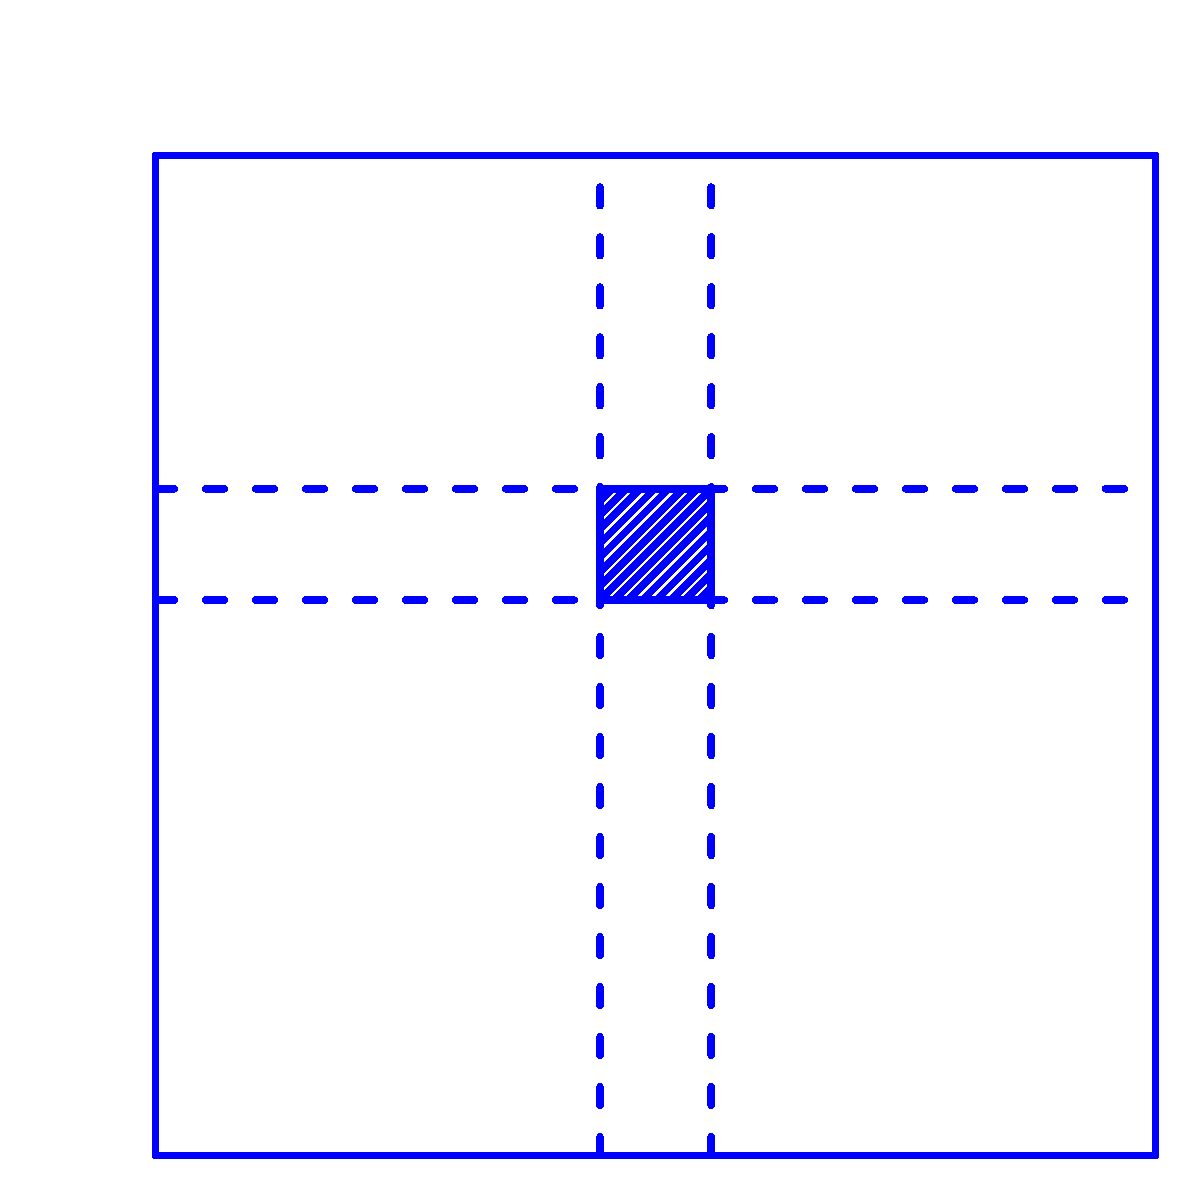
\includegraphics[scale = 0.16]{./plots/tensor.pdf}
            %\put(-2.8,2.6){\tiny $\varphi(x)\otimes\psi(\yb)$}
            \put(-100,50){\tiny $\varphi(x_i)$}
            \put(-45,85){\tiny $\psi(\yb_i)$}
            \put(-40,40){\tiny $\varphi(x_i)^T\psi(\yb_i)$}
            \end{picture}
        \end{column}
    \end{columns}
    \end{itemize}
\end{itemize}
\end{frame}

\begin{frame}[allowframebreaks]{Max-Margin Conditional Random Field}{Compatibility Function}
\begin{itemize}
    \item Model family
    \begin{itemize}
        \item Exponential family defined on Markov network $\Gcal=(\Ecal, \Vcal)$:
        \begin{align*}
        P(\yb|x) = \frac{1}{Z(x,\wb)}\prod_{e\in\Ecal}{\exp(\wb_e^T\phi_e(x,\yb_e))},
        \end{align*}
        which leads to a log linear model:
        \begin{align*}
        \log P(\yb|x) = \wb^T\phi(x_i,\yb_i) - \log Z(x,\wb).
        \end{align*}
    \end{itemize}
    \framebreak
    \item {Margin-based learning:}
    \begin{itemize}
        \item Use margin-based learning to avoid partition function $Z(\wb,x)$
        \item Related to odds-ratio learning:
        \begin{align*}
        \frac{\log P(\yb_i|x_i)}{\log P(\yb|x_i)} = \wb^T\phi(x_i,\yb_i) - \wb^T\phi(x_i,\yb)
        \end{align*}
        Maximize the margin between real example $\phi(x_i,\yb_i)$ and all the pseudo-example $\phi(x_i,\yb)$, according to $\ell_\Delta(\yb_i,\yb)$. 
    \end{itemize}
    \item Compatibility Function
    \begin{align*}
        F(x_i,\yb_i;\wb) &= \wb^T\phi(x_i,\yb_i)
    \end{align*}
\end{itemize}
\end{frame}

\begin{frame}{Max-Margin Conditional Random Field}{Maximum Margin Learning}
\begin{itemize}
    \item Maximize the margin of difference in compatibility score between correct pair and incorrect pair
    \item Optimization problem (quadratic programming)
    \begin{columns}
        \begin{column}{.3\linewidth}
            \begin{align*}
            (\wb) =& \underset{w,\xi\ge0}{\operatorname{\argmin}}\left(\frac{1}{2}||\wb||^2+C\sum_{i=1}^{n}{\xi_i}\right)\\
            \textbf{s.t.} & \, \wb^T\phi(x_i,\yb_i)-\wb^T\phi(x_i,\yb)\\
            & \ge\ell_\Delta(\yb_i,\yb)-\xi_i, \, \forall x_i,\yb.
            \end{align*}
        \end{column}
        \begin{column}{.3\linewidth}
        \begin{figure}
        \only<1>{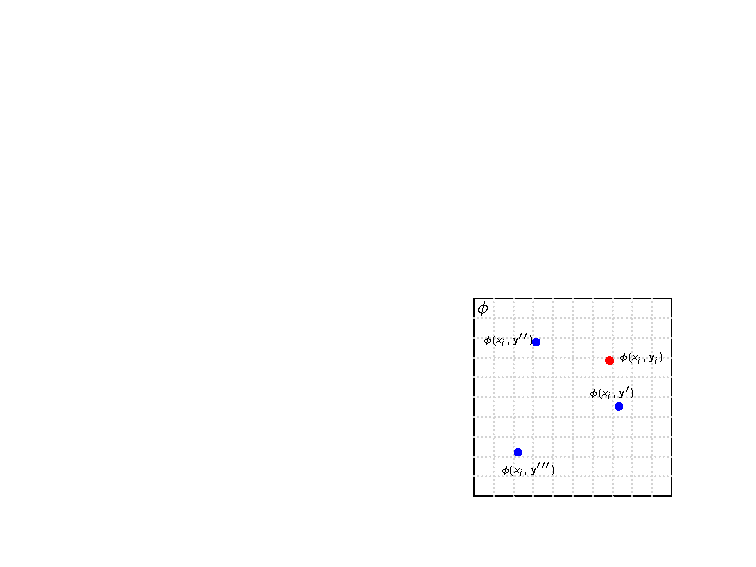
\includegraphics[scale=1]{./plots/mm0.pdf}}
        \only<2>{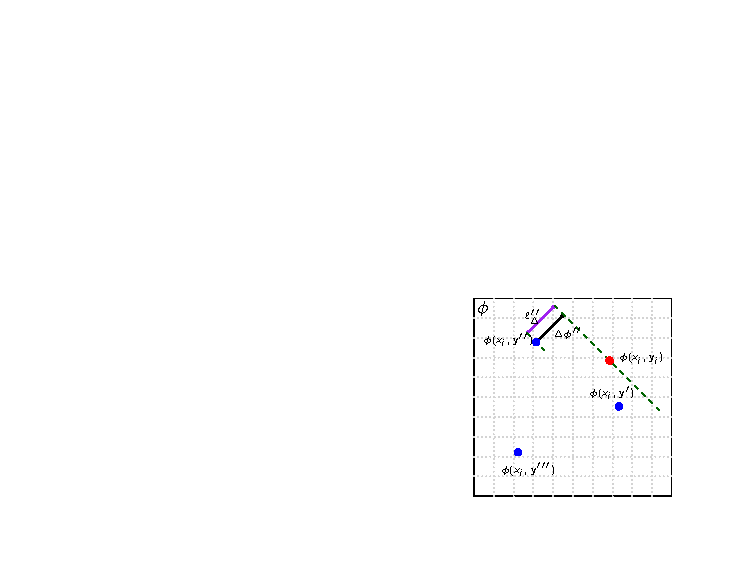
\includegraphics[scale=1]{./plots/mm1.pdf}}
        \only<3>{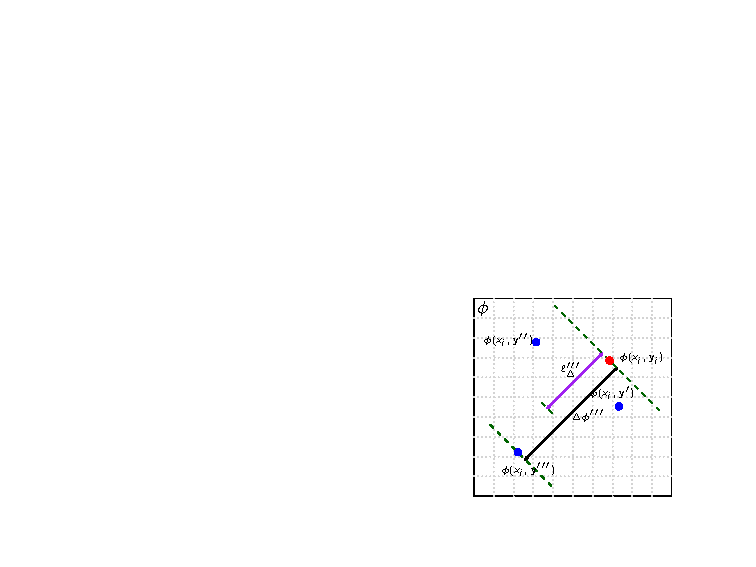
\includegraphics[scale=1]{./plots/mm2.pdf}}
        \only<4>{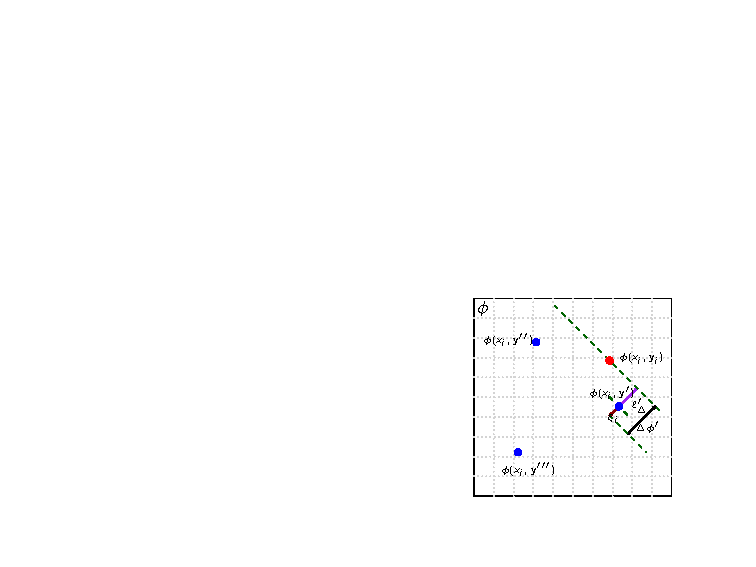
\includegraphics[scale=1]{./plots/mm3.pdf}}
        \only<5>{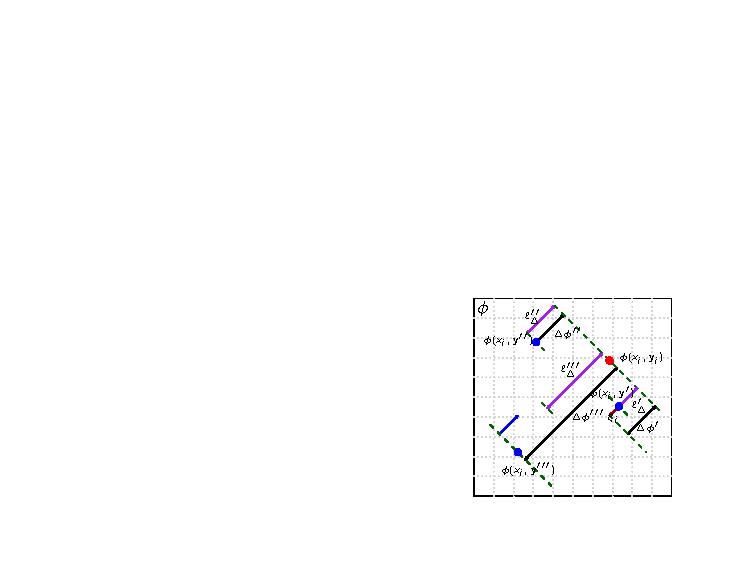
\includegraphics[scale=1]{./plots/mm4.pdf}}
        \end{figure}
        \end{column}
    \end{columns}
\end{itemize}
\end{frame}

\begin{frame}{Max-Margin Conditional Random Field}{Prediction}
\begin{itemize}
    \item Prediction is made by
    \begin{align*}
        \yb^* = \underset{\yb\in\mathcal{Y}}{\argmax} \, \wb^T\phi(x_i,\yb_i)
    \end{align*}
\end{itemize}
\end{frame}


%\begin{frame}{Summary}
%\begin{itemize}
    %\item 
%\end{itemize}
%\end{frame}

%\begin{frame}{Introduction}
%\begin{itemize}
%\item The purpose of \texttt{aaltoslides} is to allow us who use Beamer to easily produce slides that somewhat look like the official Aalto slides
%\item \texttt{aaltoslides} has \alert{not} been approved by anybody responsible of the Aalto visual style
%\item \texttt{aaltoslides} only resembles the official Aalto Powerpoint templates: font (Helvetica, not Nimbus Sans), sizes of the logos, footer bars, etc. may differ from the official ones
%\item All comments are welcome! (kimmo.jarvinen@tkk.fi)
%\end{itemize}
%\end{frame}

%%%%%%%%%%%%%%%%%%%%%%%%%%%%%%%%%%%%%%%%%%%%%%%%%%%%%%%%%%%%%%%%%%%%%%%%%%%%%%%%%%%%%%%%%%%%%%%
%%%%%%%%%%%%%%%%%%%%%%%%%%%%%%%%%%%%%%%%%%%%%%%%%%%%%%%%%%%%%%%%%%%%%%%%%%%%%%%%%%%%%%%%%%%%%%

%\begin{frame}{Title Page}

%\begin{itemize}
%\item The largest difference to normal Beamer slides is that the title page is produced with a special command \texttt{\textbackslash aaltotitleframe}; this command should be used as it is. \alert{Don't put it in a frame environment!!!} See \texttt{example.tex}.
%\item By default, \texttt{aaltoslides} uses a title page similar to the one in the Aalto Powerpoint templates
%\item A more traditional looking title page can be selected with the option: \texttt{normaltitle}
%\end{itemize}

%\end{frame}

%%%%%%%%%%%%%%%%%%%%%%%%%%%%%%%%%%%%%%%%%%%%%%%%%%%%%%%%%%%%%%%%%%%%%%%%%%%%%%%%%%%%%%%%%%%%%%

%\begin{frame}{Aalto Colors}

%\begin{itemize}

%\item Colors are defined with options: \texttt{first=$\star$} and \texttt{second=$\star$} where $\star$ is one of the following:\\
%{\color{aaltoyellow}yellow}, 
%{\color{aaltored}red}, 
%{\color{aaltoblue}blue}, 
%{\color{aaltogray}gray}, 
%{\color{aaltolgreen}lgreen}, 
%{\color{aaltodgreen}dgreen}, 
%{\color{aaltocyan}cyan}, 
%{\color{aaltopurple}purple}, 
%{\color{aaltomagenta}magenta}, or
%{\color{aaltoorange}orange}

%\item The first color is the primary color (titles, the footer bar, \ldots) and the second color is used in alerted texts and examples

%\item Default colors are: {\color{aaltoblue}blue} and {\color{aaltored}red}

%\item Colors can be used also with the command: \texttt{\textbackslash color\{aalto}$\star$\texttt{\}}. For example, 
%\texttt{\{\textbackslash color\{aaltocyan\}some text\}} 
%gives {\color{aaltocyan}some text}

%\item The rules for choosing colors from the Aalto color circle are not checked (two adjacent colors should not be used)

%\end{itemize}

%\end{frame}

%%%%%%%%%%%%%%%%%%%%%%%%%%%%%%%%%%%%%%%%%%%%%%%%%%%%%%%%%%%%%%%%%%%%%%%%%%%%%%%%%%%%%%%%%%%%%%

%\begin{frame}{Logo}

%\begin{itemize}
%\item \texttt{aaltoslides} supports all variations of the logo:\\[0.2cm]
%
\includegraphics[width=3cm]{Aalto_EN_ScienceandTech_13_RGB_y1.pdf} \hspace{10pt}
%
\includegraphics[width=3cm]{Aalto_EN_ScienceandTech_13_RGB_y2.pdf} \hspace{10pt}
%
\includegraphics[width=3cm]{Aalto_EN_ScienceandTech_13_RGB_y3.pdf} \\[0.2cm]
%
\includegraphics[width=3cm]{Aalto_EN_ScienceandTech_13_RGB_r1.pdf} \hspace{10pt}
%
\includegraphics[width=3cm]{Aalto_EN_ScienceandTech_13_RGB_r2.pdf} \hspace{10pt}
%
\includegraphics[width=3cm]{Aalto_EN_ScienceandTech_13_RGB_r3.pdf} \\[0.2cm]
%
\includegraphics[width=3cm]{Aalto_EN_ScienceandTech_13_RGB_b1.pdf} \hspace{10pt}
%
\includegraphics[width=3cm]{Aalto_EN_ScienceandTech_13_RGB_b2.pdf} \hspace{10pt}
%
\includegraphics[width=3cm]{Aalto_EN_ScienceandTech_13_RGB_b3.pdf} \\
%\item The logo is selected with the option: \texttt{logo=$\star\circ$} where $\star$ is {\color{aaltoyellow}yellow}, {\color{aaltored}red}, or {\color{aaltoblue}blue}, and $\circ$ is either exc, quo, or que for !, ", or ?, respectively; For example, \texttt{logo=yellowquo}
%\item The title page uses a larger variation of the selected logo
%\item By default, the logo is \texttt{logo=redexc}
%\item All logos can be removed with the option: \texttt{nologo}
%\end{itemize}

%\end{frame}

%%%%%%%%%%%%%%%%%%%%%%%%%%%%%%%%%%%%%%%%%%%%%%%%%%%%%%%%%%%%%%%%%%%%%%%%%%%%%%%%%%%%%%%%%%%%%%

%\begin{frame}{Footer}

%\begin{itemize}

%\item By default, the slides have a footer with a logo on the left and an optional three row text\footnote{The first row is highlighted with black by default. To remove this, simply change the color of the first argument of  \texttt{\textbackslash aaltofootertext\{\}\{\}\{\}} with \texttt{\textbackslash color\{aaltogray\}}} on the right
%\item The footer text is set up with the command: \texttt{\textbackslash aaltofootertext\{\}\{\}\{\}}
%\item The footer can be removed with the option: \texttt{nofoot}

%\end{itemize}

%\end{frame}

%%%%%%%%%%%%%%%%%%%%%%%%%%%%%%%%%%%%%%%%%%%%%%%%%%%%%%%%%%%%%%%%%%%%%%%%%%%%%%%%%%%%%%%%%%%%%%

%\begin{frame}{Lengths}

%\begin{itemize}
%\item \texttt{aaltoslides} defines the following lengths: 
%\texttt{\textbackslash aaltofooterplace}, 
%\texttt{\textbackslash aaltofooterruleheight}, 
%\texttt{\textbackslash aaltofooterrulewidth}, 
%\texttt{\textbackslash aaltotitleboxplace},  
%\texttt{\textbackslash aaltotitleboxheight}, 
%\texttt{\textbackslash aaltotitleboxwidth}, 
%\texttt{\textbackslash aaltotitlesep}, 
%\texttt{\textbackslash aaltotitleentrysep}, 
%\texttt{\textbackslash largelogoheight}, and
%\texttt{\textbackslash smalllogoheight} 
%\item The appearance of the slides can be changed by modifying the lengths with \texttt{\textbackslash setlength} or \texttt{\textbackslash addtolength}
%\end{itemize}

%\end{frame}

%%%%%%%%%%%%%%%%%%%%%%%%%%%%%%%%%%%%%%%%%%%%%%%%%%%%%%%%%%%%%%%%%%%%%%%%%%%%%%%%%%%%%%%%%%%%%%


%\begin{frame}{Some Examples}

%\begin{itemize}
%\item Normal text
%\item \alert{Alerted text}
%\end{itemize}

%\begin{block}{Block 1}
%Text
%\end{block}

%\begin{example}
%Text
%\end{example}

%\end{frame}

\begin{frame}[allowframebreaks]{Bibliography}
%\bibliographystyle{plain}
\bibliographystyle{apalike}
 \bibliography{example}
\end{frame}

%%%%%%%%%%%%%%%%%%%%%%%%%%%%%%%%%%%%%%%%%%%%%%%%%%%%%%%%%%%%%%%%%%%%%%%%%%%%%%%%%%%%%%%%%%%%%
\end{document}
